\chapter{再生核Hilbert空间}
\label{chap:rkhs}

设想我们在区间上布置了几个传感器，只能读出未知函数在这些位置的取值。要把这些读数当作关于函数的可靠信息，至少需要两件事：函数本身改动一点时，读数只改动一点；读数背后对应的函数方向要能具体写出来。第~\ref{chap:linear-functionals-operators}章已经看到，在$L^2$这样的积分空间里，单点取值往往连定义都没有；即便限制为连续函数，平方积分很小的函数也可能在某一点取值很大。另一方面，第~\ref{chap:weak-derivatives-sobolev}章中一维Sobolev函数有连续代表，点值受Sobolev范数控制。本章研究的正是这一类空间：由真实函数组成、点值读取连续的Hilbert空间。

本章要回答四个相互衔接的问题。第一，点值连续时，每个点的读取能否写成与某个固定函数的内积，这些函数合在一起记录了什么？第~\ref{sec:rkhs-point-evaluation}节用Riesz表示得到再生核，并说明核怎样同时刻画单点读取的强弱与读数随位置变化的方式。第二，能否反过来只给定一个二元函数就确定空间？第~\ref{sec:rkhs-construction}节从半正定核出发构造空间，再给出特征映射与核运算两种可检查的构造途径。第三，只拿到有限个点值时，函数的哪些部分被看见、哪些部分完全看不见？第~\ref{sec:rkhs-finite-observations}节用正交投影回答这个问题，并把有限维计算写成核矩阵。第四，若在输入集上再给定一个测度，核积分算子的谱能否提供另一种正交表示？第~\ref{sec:rkhs-spectral}节建立Mercer展开，比较两种范数的谱权重，并对比按谱截断与按观测中心投影得到的两种有限表示。

前两节只用到集合、Hilbert空间与有界线性泛函，不需要测度；测度只在最后一节出现，用来产生积分算子与新的正交坐标。全章约定函数取实值，输入集$X$是非空集合，没有额外说明时不要求它带距离或测度。三个例子贯穿全章：仿射核$K(x,z)=1+xz$给出二维空间，便于逐个坐标核对；$[0,1]$上的最小值核$K(x,z)=\min(x,z)$给出与一维Sobolev空间相连的无限维空间；高斯核则代表光滑且严格正定的核。如何用核截面逼近一般连续函数、如何用有限个代表覆盖整类函数，留到第~\ref{chap:function-approximation}章讨论。

% 第5章第1节：点值与再生核（点值泛函与再生关系、再生核的性质）。

\section{点值与再生核}
\label{sec:rkhs-point-evaluation}

本节固定一个由真实函数组成的Hilbert空间，要求每个点的取值都连续地依赖于函数。第~\ref{sec:lfo-point-evaluation}节已经把点值读取的良定义与有界性分开讨论；这里把两项要求同时作为空间的前提，再用第~\ref{sec:lfo-riesz}节的Riesz表示把每个点的读取写成内积。由此得到的二元函数称为再生核。第~\ref{sec:rkhs-kernel-properties}节再从核本身读出点值的强弱、核矩阵的符号，以及读数随位置变化的方式。

\subsection{点值泛函与再生关系}
\label{sec:rkhs-reproducing}
\label{subsubsec:point-evaluation}

\paragraph{点值读取的两项要求}

回顾第~\ref{sec:lfo-point-evaluation}节的两个反例。在Lebesgue测度下，$L^2[0,1]$的元素是几乎处处相等的函数类，零函数与只在$x=1/2$处取$1$的函数属于同一类，却给出不同的点值，所以“取$1/2$处的值”在$L^2$上没有良定义。即使只考虑连续函数，尖峰$f_n(t)=\max(1-nt,0)$满足$\|f_n\|_{L^2}^2=1/(3n)$而$f_n(0)=1$，比值$f_n(0)/\|f_n\|_{L^2}=\sqrt{3n}$没有上界，原点的读取不受$L^2$范数控制。

这两个反例说明，点值要成为可靠的信息，空间必须同时满足两条：元素是真正的函数，每个$f(x)$都有确定的数值；并且对每个固定的$x$，读取$f\mapsto f(x)$是有界线性泛函。第一条由空间的选取保证，第二条则依赖空间所带的范数。下面的例子同时满足两条，它会在本章反复出现。

\paragraph{一个满足两项要求的空间}

令$H_{\min}$为$[0,1]$上满足$f(0)=0$、几乎处处导数$f'\in L^2(0,1)$的绝对连续函数全体，内积取
\[
\langle f,g\rangle_{H_{\min}}=\int_0^1f'(t)g'(t)\,\mathrm dt .
\]
绝对连续保证$f(x)=\int_0^xf'(t)\,\mathrm dt$，所以映射$f\mapsto f'$把$H_{\min}$一一地映到$L^2(0,1)$上，逆映射是$g\mapsto\int_0^{\,\cdot}g$，并且保持内积。由此，$\langle f,f\rangle=0$迫使$f'=0$几乎处处，再由$f(0)=0$得$f=0$；$L^2(0,1)$的完备性也随这个等距对应传到$H_{\min}$。这些函数正是第~\ref{sec:sob-absolute-continuity}节中$H^1(0,1)$元素的连续代表里左端取零的那一部分。

在$H_{\min}$中读取一点的值，只需对导数作Cauchy--Schwarz估计：
\begin{equation}
|f(x)|=\Bigl|\int_0^x f'(t)\,\mathrm dt\Bigr|
\le\Bigl(\int_0^x1\,\mathrm dt\Bigr)^{1/2}\|f'\|_{L^2}
=\sqrt x\,\|f\|_{H_{\min}} .
\label{eq:rkhs-hmin-point-bound}
\end{equation}
因此每个点的读取都有界，常数$\sqrt x$随位置变化，在整个区间上不超过$1$。这与第~\ref{sec:sob-embedding}节一维Sobolev函数的点值估计是同一个机制：导数的平方积分控制了函数沿路径的累计变化，再由左端的固定值得到点值。

\paragraph{再生核Hilbert空间的定义}

把上述两项要求抽象出来，就得到本章的研究对象。

\begin{definition}[再生核Hilbert空间]
\label{def:rkhs-rkhs}
设$X$是非空集合，$H$是由函数$f:X\to\mathbb R$组成的实Hilbert空间，其加法与数乘按逐点方式定义。若对每个$x\in X$，\term{点值泛函}（evaluation functional）$L_x:H\to\mathbb R$，$L_x(f)=f(x)$都是有界线性泛函，则称$H$为\term{再生核Hilbert空间}（reproducing kernel Hilbert space，RKHS）。
\end{definition}

定义中逐点运算这一条不能省略：它保证$H$的零元就是处处为零的函数，从而“两个元素相等”与“两个函数在每一点取值相同”是同一件事。$L^2$的元素不是这样的函数，所以它不在定义的讨论范围之内，这与它的点值读取没有良定义是一致的。

对每个$x$，$L_x$有界且$H$是Hilbert空间，第~\ref{sec:lfo-riesz}节的Riesz表示给出唯一的$K_x\in H$，使得
\begin{equation}
f(x)=\langle f,K_x\rangle_H\qquad(f\in H),
\label{eq:rkhs-reproducing}
\end{equation}
并且$\|L_x\|=\|K_x\|_H$。$K_x$本身也是$X$上的函数。定义二元函数
\begin{equation}
K(z,x)=K_x(z)=\langle K_x,K_z\rangle_H\qquad(x,z\in X),
\label{eq:rkhs-kernel-definition}
\end{equation}
其中第二个等号是对$f=K_x$在点$z$处使用式~\eqref{eq:rkhs-reproducing}。称$K$为$H$的\term{再生核}（reproducing kernel），称$K_x=K(\cdot,x)$为核在$x$处的\term{核截面}（kernel section）。式~\eqref{eq:rkhs-reproducing}称为\term{再生性质}（reproducing property）：在$x$处读取$f$，等于拿$f$与固定函数$K_x$作内积；把$f$换成$K_z$，读出的又是核本身的值，“再生”一词即由此而来。

\paragraph{仿射函数空间中的核验}

最小的非平凡例子是仿射函数空间
\[
H_{\mathrm{aff}}=\{f(t)=a+bt:\ a,b\in\mathbb R\},\qquad
\langle a+bt,\ a'+b't\rangle=aa'+bb' ,
\]
输入集取$X=\mathbb R$。这个内积就是系数向量的欧氏内积，所以$H_{\mathrm{aff}}$是二维Hilbert空间。我们来找$K_x$：它应是某个仿射函数$c+dt$，满足$\langle a+bt,c+dt\rangle=ac+bd=a+bx$对一切$a,b$成立，于是$c=1$、$d=x$，即
\[
K_x(t)=1+xt,\qquad K(t,x)=1+xt .
\]
逐项核对再生性质：$\langle a+bt,K_x\rangle=a\cdot1+b\cdot x=f(x)$。

图~\ref{fig:rkhs-reproducing-geometry}把这个计算画在系数平面上。由于系数平面与$H_{\mathrm{aff}}$等距，每个核截面$K_x$对应向量$(1,x)$，它们全都落在竖直直线$a=1$上。读取$f=1+t$在$x=1/2$处的值，就是计算$(1,1)$与$(1,1/2)$的内积$1.5$；而$K_{-1}=(1,-1)$与$(1,1)$正交，对应$f(-1)=0$。一个函数在某点取零，几何上就是它与该点的核截面垂直。

\begin{figure}[!htb]
  \centering
  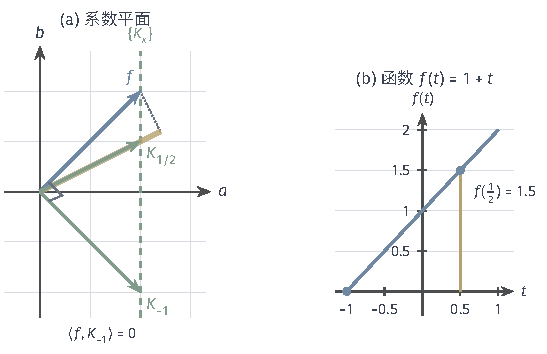
\includegraphics[width=92.7mm]{figures/02-abstract-mathematics/03-function-spaces/tikz/c5-reproducing-geometry/figure.pdf}
  \caption{仿射函数空间中再生性质的几何。(a)~系数平面$(a,b)$与空间等距；$f=1+t$对应$(1,1)$，核截面$K_x=1+xt$对应$(1,x)$，都落在虚线$a=1$上。黄色线段是$f$在$K_{1/2}$方向上的投影，其长度乘以$\|K_{1/2}\|$等于$f(1/2)=1.5$；$K_{-1}$与$f$垂直。(b)~同一函数的图像，标出$t=1/2$处的读数$1.5$与$t=-1$处的零点。}
  \label{fig:rkhs-reproducing-geometry}
\end{figure}

\paragraph{最小值核}

在$H_{\min}$中，核截面同样可以直接猜出来。式~\eqref{eq:rkhs-hmin-point-bound}的推导把$f(x)$写成了$\int_0^1f'(t)\mathbf 1_{[0,x]}(t)\,\mathrm dt$，所以只需找一个导数为$\mathbf 1_{[0,x]}$、左端取零的函数，它就是
\[
K_x(t)=\min(t,x),\qquad K(t,x)=\min(t,x)\qquad(t,x\in[0,1]).
\]
$K_x$在$[0,x]$上斜率为$1$，在$[x,1]$上保持常数$x$，确实属于$H_{\min}$，并且$\langle f,K_x\rangle_{H_{\min}}=\int_0^xf'(t)\,\mathrm dt=f(x)$。称$K(x,z)=\min(x,z)$为$[0,1]$上的\term{最小值核}（minimum kernel）。它在概率论中是标准Brown运动的协方差，但这里只把它当作一个确定的二元函数使用。

\paragraph{逐点常数与统一常数}

定义只要求每个$L_x$有界，有界常数$\|L_x\|$允许随$x$变化。在$H_{\mathrm{aff}}$中，$\|L_x\|=\|K_x\|=\sqrt{1+x^2}$。所以单位球中的函数在$x$处的取值恰好填满区间$[-\sqrt{1+x^2},\sqrt{1+x^2}]$：上界由Cauchy--Schwarz不等式给出，取$f=K_x/\|K_x\|$即可达到。

图~\ref{fig:rkhs-pointwise-envelope}画出这条包络和几条单位范数函数$\cos\theta+t\sin\theta$。每条函数在$t=\tan\theta$处与上包络相切，这正是它与$K_t$同向的位置。在整条实轴上，包络随$|t|$无限增长，不存在统一的常数$C$使$|f(t)|\le C\|f\|$对一切$t$成立；若把输入集限制为$[-1,1]$，统一常数就是$\sqrt2$。一般地，只有当$\sup_{x\in X}K(x,x)<\infty$时，核范数才能统一控制全域的点值误差：
\[
\sup_{x\in X}|f(x)-g(x)|\le\Bigl(\sup_{x\in X}\sqrt{K(x,x)}\Bigr)\,\|f-g\|_H .
\]
对$H_{\min}$，由式~\eqref{eq:rkhs-hmin-point-bound}，统一常数是$1$。

\begin{figure}[!htb]
  \centering
  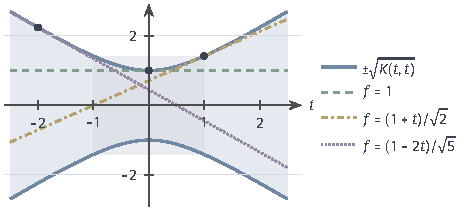
\includegraphics[width=79.6mm]{figures/02-abstract-mathematics/03-function-spaces/tikz/c5-pointwise-envelope/figure.pdf}
  \caption{仿射函数空间单位球在各点的取值范围。浅蓝区域介于$\pm\sqrt{K(t,t)}=\pm\sqrt{1+t^2}$之间；三条虚线是单位范数函数，各自在黑点处与上包络相切。灰色区域标出$[-1,1]$，其中包络的最大值为$\sqrt2$。包络在整条实轴上无界，说明逐点有界不等于统一有界。}
  \label{fig:rkhs-pointwise-envelope}
\end{figure}

\paragraph{离散空间也是RKHS}

再看一个点值有界、函数却毫无连续性的例子。对任意非空集合$X$，令$\ell^2(X)$为满足$\sum_{x\in X}f(x)^2<\infty$的函数全体（求和对至多可数个非零项进行），内积为$\sum_xf(x)g(x)$。显然$|f(x)|\le\|f\|$，所以它是RKHS，其核截面是单点示性函数$K_x=\mathbf 1_{\{x\}}$，再生核是$K(x,z)=1$（$x=z$）或$0$（$x\neq z$）。即使$X=[0,1]$，这个空间中的函数也可以在每点任意跳动。可见点值有界只是对每个固定位置的要求，函数是否随位置连续，需要核提供更多信息。

\subsection{再生核的性质}
\label{sec:rkhs-kernel-properties}

上一小节从空间得到了核。核是一个具体的二元函数，下面看它从三个方面记录空间的信息：每点读取的强弱、任意有限点组上核值矩阵的符号，以及读数随位置的变化。

\paragraph{对称性、半正定性与点值范数}

由定义式~\eqref{eq:rkhs-kernel-definition}，核值是两个核截面的内积，因此内积的性质直接转化为核的性质。

\begin{theorem}[再生核的基本性质]
\label{thm:rkhs-kernel-properties}
设$H$是$X$上的RKHS，$K$为其再生核。则：
\begin{enumerate}
\item 对称性：$K(x,z)=K(z,x)$对一切$x,z\in X$成立；
\item 半正定性：对任意$n\ge1$、任意点$x_1,\ldots,x_n\in X$与实数$a_1,\ldots,a_n$，
\[
\sum_{i,j=1}^na_ia_jK(x_i,x_j)=\Bigl\|\sum_{i=1}^na_iK_{x_i}\Bigr\|_H^2\ge0 ;
\]
\item 点值范数：$\|L_x\|=\|K_x\|_H=\sqrt{K(x,x)}$；并且对任意$x,z\in X$，$|K(x,z)|\le\sqrt{K(x,x)K(z,z)}$。
\end{enumerate}
\end{theorem}

\begin{proof}
由式~\eqref{eq:rkhs-kernel-definition}，$K(x,z)=\langle K_z,K_x\rangle$，实内积的对称性给出第1条。把$\bigl\|\sum_ia_iK_{x_i}\bigr\|^2$按双线性展开为$\sum_{i,j}a_ia_j\langle K_{x_i},K_{x_j}\rangle$，再用$\langle K_{x_i},K_{x_j}\rangle=K(x_j,x_i)=K(x_i,x_j)$，得到第2条。Riesz表示给出$\|L_x\|=\|K_x\|$，而$\|K_x\|^2=\langle K_x,K_x\rangle=K(x,x)$。最后，$|K(x,z)|=|\langle K_z,K_x\rangle|\le\|K_z\|\|K_x\|$。
\end{proof}

第2条中的矩阵$\bm G=[K(x_i,x_j)]_{i,j=1}^n$称为点组$x_1,\ldots,x_n$上的\term{Gram矩阵}或\term{核矩阵}（kernel matrix）。第2条说的就是：每个Gram矩阵都是对称半正定矩阵。这一性质不依赖于空间，只依赖于核，因此可以单独作为对二元函数的要求。

\begin{definition}[半正定核与严格正定核]
\label{def:rkhs-psd-kernel}
设$X$是非空集合。若函数$K:X\times X\to\mathbb R$对称，且对任意有限点组，其Gram矩阵都半正定，则称$K$为$X$上的半正定核，文献中也常称为\term{正定核}（positive definite kernel）。若对任意互异点$x_1,\ldots,x_n$及任意不全为零的实数$a_1,\ldots,a_n$都有$\sum_{i,j}a_ia_jK(x_i,x_j)>0$，即互异点上的Gram矩阵都可逆，则称$K$为\term{严格正定核}（strictly positive definite kernel）。
\end{definition}

“正定核”这个通行名称容易引起误解：它允许Gram矩阵奇异。本书在需要强调时写“半正定核”，与严格正定的情形区分。

\paragraph{仿射核的奇异Gram矩阵}

仿射核说明这种区分是必要的。取三个点$-1,0,1$，Gram矩阵与一个零向量为
\[
\bm G=\begin{bmatrix}2&1&0\\1&1&1\\0&1&2\end{bmatrix},\qquad
\bm G\begin{bmatrix}1\\-2\\1\end{bmatrix}=\bm 0 .
\]
对应的函数组合$K_{-1}-2K_0+K_1=(1-t)-2+(1+t)$恰好是零函数。原因很直接：$H_{\mathrm{aff}}$只有二维，任意三个核截面必然线性相关。图~\ref{fig:rkhs-gram-matrices}对五个点比较了两种核：高斯核$K(x,z)=\exp\bigl(-(x-z)^2/(2\sigma^2)\bigr)$（$\sigma=0.5$）的Gram矩阵五个特征值都为正，仿射核的Gram矩阵则只有两个正特征值$5$与$2.5$，其余三个为零。两者都是半正定核，只有前者在这个点组上可逆。

\begin{figure}[!htb]
  \centering
  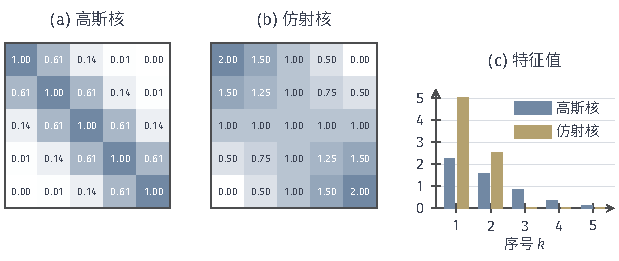
\includegraphics[width=104.8mm]{figures/02-abstract-mathematics/03-function-spaces/tikz/c5-gram-matrices/figure.pdf}
  \caption{点组$x=-1,-0.5,0,0.5,1$上的Gram矩阵。(a)~高斯核（$\sigma=0.5$），颜色越深核值越大，数字保留两位小数（右上角的$0.00$实为$e^{-8}\approx0.0003$）；(b)~仿射核$1+xz$；(c)~两个矩阵的特征值。高斯核的特征值$2.217,1.531,0.820,0.333,0.099$全为正；仿射核只有$5$与$2.5$两个正特征值，其余为零。两种核都半正定，只有前者的矩阵可逆。}
  \label{fig:rkhs-gram-matrices}
\end{figure}

高斯核在任意有限个互异实数上都给出可逆Gram矩阵，即它是严格正定核。这一结论的证明需要Fourier变换，这里不展开；本章后面用到高斯核时，只在具体计算中检查相应矩阵的可逆性。严格正定性与半正定性是两项不同的要求：半正定性可由第~\ref{sec:rkhs-kernel-operations}节的运算规则逐步验证，严格正定性则须对互异点组另行判断。

\paragraph{核截面的形状}

核截面$K_x$是$H$中的元素，所以它的形状直接展示了空间中函数的样子。图~\ref{fig:rkhs-kernel-sections}画出三种核在$[-1,1]$上的截面。高斯核的截面是以$x$为中心的钟形，离$x$越远取值越小；仿射核的截面是过点$(0,1)$的直线；二次多项式核$(1+xt)^2$的截面是抛物线。后两种核的截面都只在有限维函数族中变化，它们张成的空间分别是仿射函数与至多二次的多项式；高斯核截面则彼此不在任何有限维子空间中，这与它的严格正定性相符。

\begin{figure}[!htb]
  \centering
  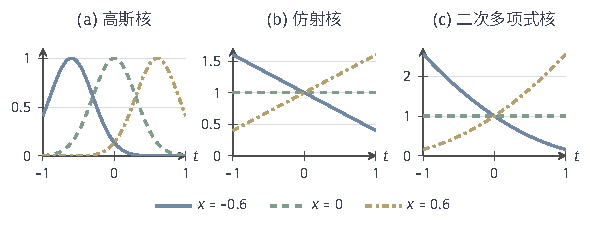
\includegraphics[width=99.9mm]{figures/02-abstract-mathematics/03-function-spaces/tikz/c5-kernel-sections/figure.pdf}
  \caption{三种核在$[-1,1]$上的核截面$K_x(t)=K(t,x)$，$x=-0.6,0,0.6$。(a)~高斯核（$\sigma=0.3$），截面是以$x$为中心的钟形；(b)~仿射核$1+xt$，截面是直线；(c)~二次多项式核$(1+xt)^2$，截面是抛物线。核截面是空间中的元素，其形状展示了空间所含函数的类型。}
  \label{fig:rkhs-kernel-sections}
\end{figure}

\paragraph{位置变化与核截面的距离}

到目前为止，每个点的读取是分开讨论的。现在固定函数$f$，只移动读取位置。由再生性质，
\[
f(x)-f(z)=\langle f,K_x-K_z\rangle_H ,
\]
所以
\begin{equation}
\begin{gathered}
|f(x)-f(z)|\le\|f\|_H\,\|K_x-K_z\|_H,\\
\|K_x-K_z\|_H^2=K(x,x)+K(z,z)-2K(x,z) .
\end{gathered}
\label{eq:rkhs-position-bound}
\end{equation}
第二个等式由展开$\langle K_x-K_z,K_x-K_z\rangle$并使用式~\eqref{eq:rkhs-kernel-definition}得到。式~\eqref{eq:rkhs-position-bound}把位置的变化转化为两个核截面在$H$中的距离，而这个距离只用核的三个值就能算出。

对三个例子分别计算这个距离。高斯核满足$K(x,x)=1$，于是$\|K_x-K_z\|^2=2-2e^{-d^2/(2\sigma^2)}$，其中$d=|x-z|$；由$1-e^{-u}\le u$得$\|K_x-K_z\|\le d/\sigma$，所以单位范数函数满足$|f(x)-f(z)|\le|x-z|/\sigma$。最小值核满足$\|K_x-K_z\|^2=x+z-2\min(x,z)=|x-z|$，于是$|f(x)-f(z)|\le\|f\|_{H_{\min}}|x-z|^{1/2}$，这正是一维Sobolev函数的$1/2$阶Hölder估计。离散空间$\ell^2(X)$的核在$x\neq z$时给出$\|K_x-K_z\|=\sqrt2$，距离不随$|x-z|$缩小。图~\ref{fig:rkhs-section-distance}把这些曲线画在一起：前两类核截面随位置连续移动，最后一类在每一点都跳开。

\begin{figure}[!htb]
  \centering
  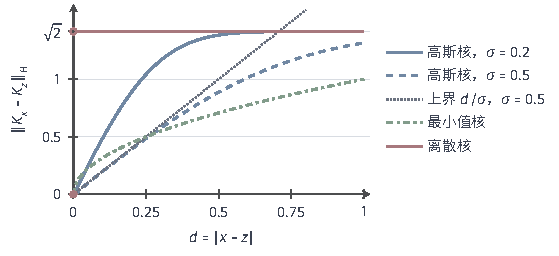
\includegraphics[width=94.7mm]{figures/02-abstract-mathematics/03-function-spaces/tikz/c5-section-distance/figure.pdf}
  \caption{核截面距离$\|K_x-K_z\|_H$随位置差$d=|x-z|$的变化。两条蓝线是高斯核（$\sigma=0.2$与$0.5$），点线是$\sigma=0.5$时的上界$d/\sigma$；绿色点划线是最小值核的$\sqrt d$；红线是离散空间$\ell^2(X)$的核，$d>0$时恒为$\sqrt2$。由式~\eqref{eq:rkhs-position-bound}，这个距离乘以$\|f\|_H$控制了$|f(x)-f(z)|$；前三条曲线在$d\to0$时趋于零，最后一条不然。}
  \label{fig:rkhs-section-distance}
\end{figure}

\paragraph{连续核与函数的连续性}

上述计算可以整理成一条一般结论。

\begin{theorem}[连续核给出连续函数]
\label{thm:rkhs-continuity}
设$X$是度量空间，$H$是$X$上的RKHS，再生核$K$在$X\times X$上连续。则：
\begin{enumerate}
\item 映射$x\mapsto K_x$从$X$到$H$连续，因而每个$f\in H$都是$X$上的连续函数；
\item 若$X$还是紧的，则对任意$R>0$，球$B_R=\{f\in H:\|f\|_H\le R\}$中的函数一致有界且等度连续：对任意$\varepsilon>0$存在$\delta>0$，使得$d(x,z)<\delta$时，对一切$f\in B_R$都有$|f(x)-f(z)|<\varepsilon$。
\end{enumerate}
\end{theorem}

\begin{proof}
当$z\to x$时，$K$的连续性使$K(z,z)\to K(x,x)$、$K(x,z)\to K(x,x)$，由式~\eqref{eq:rkhs-position-bound}的第二个等式得$\|K_x-K_z\|\to0$；再由第一个不等式，$f(z)\to f(x)$。这证明第1条。

若$X$紧，则$X\times X$紧，连续函数$K$一致连续（第~\ref{sec:metric-compact-continuous}节），并且对角线上的$K(x,x)$有最大值$M^2$。一致连续性给出：对任意$\eta>0$存在$\delta>0$，使得$d(x,z)<\delta$时$K(x,x)+K(z,z)-2K(x,z)<\eta$。取$\eta=(\varepsilon/R)^2$，式~\eqref{eq:rkhs-position-bound}便对$B_R$中所有$f$同时给出$|f(x)-f(z)|<\varepsilon$；一致有界性来自$|f(x)|\le M\|f\|\le MR$。
\end{proof}

第2条中的$\delta$只依赖于核与半径$R$，不依赖于球中具体的函数，这是“共同的连续性控制”的含义。第~\ref{sec:apx-arzela-ascoli}节将用这种一致有界、等度连续的性质判断函数族的紧性。还要强调两种稳定性的区别：固定位置时，$|f(x)-g(x)|\le\sqrt{K(x,x)}\|f-g\|_H$描述函数改变引起的读数改变；固定函数时，式~\eqref{eq:rkhs-position-bound}描述位置改变引起的读数改变。离散空间$\ell^2([0,1])$说明前者成立并不蕴含后者。

% 第5章第2节：核与函数空间的构造（从半正定核构造空间、特征映射、核的运算）。

\section{核与函数空间的构造}
\label{sec:rkhs-construction}

上一节从空间出发得到了核，并看到每个再生核都是半正定核。本节回答反方向的问题：只给定集合$X$上的一个半正定核，能否找到以它为再生核的函数空间，这个空间是否唯一。第~\ref{sec:rkhs-from-kernel}节用核截面的有限组合、商去零长度方向和完备化三步给出一般构造。一般构造虽然完整，却不便于检验一个具体的二元函数是否半正定，所以后两小节给出两种可操作的办法：把核写成特征向量的内积，或者由已知的核经运算得到新核。这些步骤都只用到集合与核，不需要预先给定测度。

\subsection{从半正定核构造空间}
\label{sec:rkhs-from-kernel}

设$K$是非空集合$X$上的半正定核。如果以$K$为再生核的空间存在，它一定含有全部核截面$K_x$，并且核截面之间的内积必须是$\langle K_x,K_z\rangle=K(z,x)$。构造就从这两点出发。

\paragraph{有限核和与它们的内积}

令$H_0=\operatorname{span}\{K_x:x\in X\}$，它由有限和$f=\sum_{i=1}^na_iK_{x_i}$组成，每个元素都是$X$上的真实函数$f(t)=\sum_ia_iK(t,x_i)$。对$f=\sum_ia_iK_{x_i}$与$g=\sum_jb_jK_{z_j}$，按照上述要求定义
\begin{equation}
\langle f,g\rangle_0=\sum_{i,j}a_ib_jK(z_j,x_i).
\label{eq:rkhs-h0-inner}
\end{equation}

同一个函数可以有多种有限和表示，必须先检查式~\eqref{eq:rkhs-h0-inner}与表示的选取无关。对$j$先求和内层的$i$，得到$\langle f,g\rangle_0=\sum_jb_jf(z_j)$，它只依赖于$f$作为函数的取值；由$K$的对称性，同一个量也等于$\sum_ia_ig(x_i)$，只依赖于$g$的取值。于是换掉$f$的表示不改变第一种写法，换掉$g$的表示不改变第二种写法，$\langle f,g\rangle_0$良定义。它显然对称、双线性，且$\langle f,f\rangle_0=\bm a^{\top}\bm G\bm a\ge0$，其中$\bm G$是点组$x_1,\ldots,x_n$上的Gram矩阵。取$g=K_x$，由第一种写法立刻得到
\begin{equation}
\langle f,K_x\rangle_0=f(x)\qquad(f\in H_0),
\label{eq:rkhs-h0-reproducing}
\end{equation}
即再生性质在$H_0$上已经成立。

\paragraph{零长度方向}

若把系数向量$\bm a$本身当作对象，二次型$\bm a^{\top}\bm G\bm a$只是半正定的，可能对非零$\bm a$取零。第~\ref{sec:rkhs-kernel-properties}节的仿射核例子中，点$-1,0,1$上的系数$(1,-2,1)$长度为零。所以不能直接把系数空间连同这个二次型当作内积空间，必须先商去零长度的方向。

把系数映成函数，恰好完成了这个商。Cauchy--Schwarz不等式的证明只用到半正定性与双线性，对$\langle\cdot,\cdot\rangle_0$同样成立，结合式~\eqref{eq:rkhs-h0-reproducing}得
\begin{equation}
|f(x)|=|\langle f,K_x\rangle_0|\le\sqrt{K(x,x)}\,\|f\|_0 .
\label{eq:rkhs-h0-point-bound}
\end{equation}
所以长度为零的组合在每一点取零，是零函数；反过来，零函数$f$满足$\langle f,f\rangle_0=\sum_ia_if(x_i)=0$。零长度的系数组合恰好就是给出零函数的组合。在仿射核的例子中，$K_{-1}-2K_0+K_1$正是零函数。因此在函数空间$H_0$上，$\langle\cdot,\cdot\rangle_0$已经是真正的内积。

\paragraph{完备化与点值的极限}

$H_0$一般不完备。为得到Hilbert空间，取$H_0$的完备化$\overline{H_0}$：由定理~\ref{thm:metric-completion}，它由$H_0$中Cauchy列的等价类组成，内积可以由连续性延拓过去（第~\ref{sec:fs-hilbert}节）。但完备化中的元素是抽象的等价类，还不是$X$上的函数，接下来要把它们变回函数。

点值估计~\eqref{eq:rkhs-h0-point-bound}正好提供了这一步。若$(f_n)$是$H_0$中的Cauchy列，则$|f_n(x)-f_m(x)|\le\sqrt{K(x,x)}\|f_n-f_m\|_0$，所以在每一点$f_n(x)$都是Cauchy数列，有确定的极限；等价的Cauchy列相差一列趋于零的函数，在每一点有相同的极限。用内积表达，就是定义
\[
J:\overline{H_0}\to\{X\text{上的实函数}\},\qquad (J\xi)(x)=\langle\xi,K_x\rangle_{\overline{H_0}} .
\]
若$f_n\to\xi$，则$f_n(x)=\langle f_n,K_x\rangle\to(J\xi)(x)$，所以$J\xi$就是逼近$\xi$的Cauchy列的逐点极限；由式~\eqref{eq:rkhs-h0-reproducing}，$J$在$H_0$上是恒等映射。

\paragraph{排除额外的零方向}

还剩一个危险：$\overline{H_0}$中两个不同的元素，会不会给出同一个函数？若是这样，函数之间就无法定义内积。等价地，要排除这样的$\xi\neq0$：$J\xi$是零函数。这一步要用到核截面在$\overline{H_0}$中稠密。若$(J\xi)(x)=\langle\xi,K_x\rangle=0$对一切$x$成立，则$\xi$与每个$K_x$正交，从而与它们的张成$H_0$正交；$H_0$在$\overline{H_0}$中稠密，所以$\xi$与整个空间正交，$\xi=0$。因此$J$是单射。

\begin{theorem}[由半正定核确定再生核Hilbert空间]
\label{thm:rkhs-moore-aronszajn}
设$K$是非空集合$X$上的半正定核。则存在唯一的RKHS，记为$H_K$，以$K$为其再生核。并且有限核和全体$H_0=\operatorname{span}\{K_x:x\in X\}$在$H_K$中稠密，$H_K$的每个元素都是$H_0$中某个Cauchy列的逐点极限。
\end{theorem}

\begin{proof}
存在性。令$H_K=J(\overline{H_0})$，并规定$\langle J\xi,J\eta\rangle_{H_K}=\langle\xi,\eta\rangle_{\overline{H_0}}$。由于$J$是线性单射，这个定义良好，且$J$成为从$\overline{H_0}$到$H_K$的等距同构，所以$H_K$是Hilbert空间；$J$的线性说明$H_K$中的加法和数乘就是逐点运算。$J$在$H_0$上是恒等映射，故$K_x=JK_x\in H_K$，并且对$f=J\xi$有
\[
f(x)=\langle\xi,K_x\rangle_{\overline{H_0}}=\langle J\xi,JK_x\rangle_{H_K}=\langle f,K_x\rangle_{H_K} .
\]
这就是以$K$为再生核的再生性质，点值有界随之成立。稠密性与逐点极限的描述来自$H_0$在$\overline{H_0}$中稠密以及上一段关于$J$的讨论。

唯一性。设$H$是另一个以$K$为再生核的RKHS。$H$含有每个$K_x$，且$\langle K_x,K_z\rangle_H=K(z,x)$，所以$H_0\subseteq H$，两者在$H_0$上的内积一致。$H_0$在$H$中也稠密：若$f\in H$与每个$K_x$正交，则由再生性质$f(x)=0$对一切$x$成立。任取$f\in H$及$H_0$中的序列$f_n\to f$（按$H$的范数），$(f_n)$是$H_0$中的Cauchy列，再生性质说明它逐点收敛到$f$；同一序列在$H_K$中收敛到其逐点极限，即$f$。所以$f\in H_K$且$\|f\|_{H_K}=\lim\|f_n\|=\|f\|_H$。对调两个空间的角色，得$H=H_K$，且范数相同。
\end{proof}

这条结论通常称为Moore--Aronszajn定理\scite{aronszajn1950kernels}。图~\ref{fig:rkhs-construction-steps}概括了四个阶段：系数组合上只有半内积；变为函数后零长度方向被商去；完备化补上极限；点值读取把极限元素重新表示为函数，核截面的稠密性保证这种表示是单射。

\begin{figure}[!htb]
  \centering
  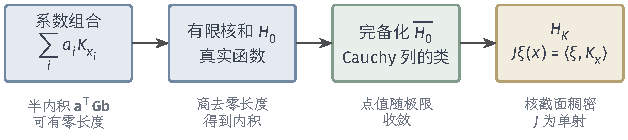
\includegraphics[width=106.4mm]{figures/02-abstract-mathematics/03-function-spaces/tikz/c5-construction-steps/figure.pdf}
  \caption{由半正定核构造$H_K$的四个阶段。系数组合上的二次型$\bm a^{\top}\bm G\bm b$只是半内积，可能有零长度方向；把组合看成函数便商去了这些方向，得到内积空间$H_0$；完备化$\overline{H_0}$的元素是Cauchy列的类，点值估计使它们的点值随极限收敛；映射$J$把它们表示为函数，核截面稠密保证$J$为单射。}
  \label{fig:rkhs-construction-steps}
\end{figure}

\paragraph{由最小值核重建$H_{\min}$}

以最小值核为例走一遍构造。$H_0$由$\min(\cdot,x_j)$的有限组合组成，即在$[0,1]$上连续、分段线性、左端为零、在最右节点之后保持常数的函数。核截面的内积可以写成导数的积分：
\[
\langle K_x,K_z\rangle_0=\min(x,z)=\int_0^1\mathbf 1_{[0,x]}(t)\mathbf 1_{[0,z]}(t)\,\mathrm dt=\int_0^1K_x'(t)K_z'(t)\,\mathrm dt ,
\]
所以在$H_0$上$\|f\|_0=\|f'\|_{L^2}$。$H_0$中函数的导数恰好是阶梯函数，而区间上的阶梯函数在$L^2(0,1)$中稠密（第~\ref{sec:fs-density-separability}节），于是完备化后得到的空间经由$f\mapsto f'$与$L^2(0,1)$等距同构，它就是第~\ref{sec:rkhs-reproducing}节的$H_{\min}$。$H_0$本身不完备：例如$f(t)=t-t^2/2$属于$H_{\min}$，却不是分段线性函数，它只是$H_0$中一列折线的极限。

这个例子也说明了唯一性的用处：我们已经知道$H_{\min}$是以$\min(x,z)$为再生核的RKHS，定理~\ref{thm:rkhs-moore-aronszajn}立刻保证从核出发构造的空间就是它，不必另作比较。

\paragraph{构造用到了什么}

整个构造只用到集合$X$与核的半正定性，没有测度，也不要求$X$带有拓扑。所得的稠密性是在核范数意义下：$H_K$中的每个函数都能被有限核和按$\|\cdot\|_{H_K}$逼近，因而也被逐点逼近。这并没有回答有限核和能否逼近$H_K$之外的函数，例如$[0,1]$上任意给定的连续函数；那是第~\ref{sec:apx-kernel-sections}节要讨论的问题，答案取决于具体的核。

\subsection{特征映射}
\label{sec:rkhs-feature-maps}

一般构造告诉我们半正定核总对应一个空间，但要验证某个二元函数半正定，逐一检查所有Gram矩阵并不现实。最常用的办法是把核写成两个向量的内积。

\paragraph{有限特征向量的内积核}

设$\Phi:X\to\mathbb R^d$，令$K(x,z)=\Phi(x)^{\top}\Phi(z)$。对任意点组与系数，
\[
\sum_{i,j}a_ia_jK(x_i,x_j)=\Bigl\|\sum_ia_i\Phi(x_i)\Bigr\|_2^2\ge0 ,
\]
所以$K$是半正定核；用矩阵写，Gram矩阵等于$\bm\Phi\bm\Phi^{\top}$，其中$\bm\Phi$的第$i$行是$\Phi(x_i)^{\top}$。例如，对实数$x,z$，
\[
(1+xz)^2=1+2xz+x^2z^2=\bigl\langle(1,\sqrt2\,x,x^2),\ (1,\sqrt2\,z,z^2)\bigr\rangle ,
\]
所以二次多项式核是三维特征向量的内积核。

\paragraph{一般特征映射}

有限维的要求可以去掉。

\begin{definition}[特征映射]
\label{def:rkhs-feature-map}
设$X$是非空集合，$\mathcal F$是实Hilbert空间，$\Phi:X\to\mathcal F$是任意映射。若$K(x,z)=\langle\Phi(x),\Phi(z)\rangle_{\mathcal F}$，则称$\Phi$为$K$的一个\term{特征映射}（feature map），$\mathcal F$为相应的特征空间。
\end{definition}

与有限维情形完全相同的计算说明，任何特征映射给出的$K$都是半正定核。反过来，每个半正定核都有特征映射：取$\mathcal F=H_K$、$\Phi(x)=K_x$，则$\langle K_x,K_z\rangle_{H_K}=K(x,z)$。称它为\term{规范特征映射}（canonical feature map）。所以“$K$半正定”与“$K$有某个特征映射”是等价的。

同一个核可以有许多不同的特征映射。仿射核$1+xz$既可以写成$\Phi_1(x)=(1,x)\in\mathbb R^2$的内积，也可以写成$\Phi_2(x)=(1,x/\sqrt2,x/\sqrt2)\in\mathbb R^3$的内积，因为$1+\tfrac{x z}{2}+\tfrac{xz}{2}=1+xz$。特征空间的维数和坐标都可以不同，核却相同，因此由核确定的空间也相同。下面说明这个空间怎样从任何一个特征映射读出来。

\paragraph{参数表示与可见子空间}

给定特征映射$\Phi:X\to\mathcal F$，每个参数$w\in\mathcal F$确定一个函数
\[
f_w(x)=\langle w,\Phi(x)\rangle_{\mathcal F}.
\]
令$V=\overline{\operatorname{span}}\{\Phi(x):x\in X\}$为特征值张成的闭子空间，$P_V$为到$V$的正交投影。由于$w-P_Vw$与每个$\Phi(x)$正交，$f_w=f_{P_Vw}$：正交补$V^\perp$中的参数分量不影响函数。称$V$为可见参数子空间。

\begin{theorem}[特征映射给出的RKHS]
\label{thm:rkhs-feature-space}
设$\Phi:X\to\mathcal F$是半正定核$K$的特征映射，$V$为特征值张成的闭子空间。则
\[
H_K=\{f_w:w\in\mathcal F\},\qquad
\|f_w\|_{H_K}=\|P_Vw\|_{\mathcal F}=\min_{u\in\mathcal F,\ f_u=f_w}\|u\|_{\mathcal F} ,
\]
并且$w\mapsto f_w$限制在$V$上是从$V$到$H_K$的等距同构。
\end{theorem}

\begin{proof}
线性映射$A:w\mapsto f_w$的核是$\{w:\langle w,\Phi(x)\rangle=0,\ \forall x\}=V^\perp$，所以$A$在$V$上是单射。令$H=A(\mathcal F)=A(V)$，并规定$\|Aw\|_H=\|P_Vw\|$，则$A|_V$是等距同构，$H$作为闭子空间$V$的等距像是Hilbert空间，运算是逐点的。

点值有界：$|f_w(x)|=|\langle P_Vw,\Phi(x)\rangle|\le\|\Phi(x)\|\,\|f_w\|_H$。再生核：令$k_x=A\Phi(x)$，因$\Phi(x)\in V$，有$\langle f_w,k_x\rangle_H=\langle P_Vw,\Phi(x)\rangle=f_w(x)$；而$k_x(z)=\langle\Phi(x),\Phi(z)\rangle=K(z,x)$，即$k_x=K_x$。所以$H$是以$K$为再生核的RKHS，由定理~\ref{thm:rkhs-moore-aronszajn}的唯一性，$H=H_K$。最后，$f_u=f_w$当且仅当$u-w\in V^\perp$，此时$P_Vu=P_Vw$，而$\|u\|\ge\|P_Vu\|$，等号在$u\in V$时取得。
\end{proof}

定理的最后一个等式提醒我们：在冗余的特征表示中，任意一个能给出$f$的参数$w$，其范数只是$\|f\|_{H_K}$的上界；只有落在可见子空间中的那一个参数，范数才等于函数的范数。

\paragraph{冗余特征的例子}

取$\Phi(x)=(x,x)\in\mathbb R^2$，核为$K(x,z)=2xz$。可见子空间是直线$V=\operatorname{span}\{(1,1)\}$，正交补方向是$(1,-1)$。参数$(2,0)$、$(1,1)$、$(0,2)$都给出同一函数$f(x)=2x$，范数分别为$2$、$\sqrt2$、$2$；由定理~\ref{thm:rkhs-feature-space}，$\|f\|_{H_K}=\sqrt2$，它是$(2,0)$在$V$上的投影$(1,1)$的长度，见图~\ref{fig:rkhs-visible-parameters}。直接检验：$H_K$由$f(x)=cx$组成，核截面$K_x(t)=2xt$，再生性质要求$\langle ct,2xt\rangle=cx$，故$\langle ct,c't\rangle_{H_K}=cc'/2$，$\|2x\|_{H_K}^2=4/2=2$，结果一致。

对仿射核的两个特征映射，$\Phi_1$的可见子空间是整个$\mathbb R^2$（$\Phi_1(-1)$与$\Phi_1(1)$线性无关），所以$\|a+bt\|_{H_K}^2=a^2+b^2$，与第~\ref{sec:rkhs-reproducing}节一致。$\Phi_2$的可见子空间是$\operatorname{span}\{(1,0,0),(0,1,1)/\sqrt2\}$，参数$(a,b/\sqrt2,b/\sqrt2)$给出$a+bt$，长度同样是$\sqrt{a^2+b^2}$；而参数$(a,\sqrt2 b,0)$给出同一函数，长度$\sqrt{a^2+2b^2}$却更大。

\begin{figure}[!htb]
  \centering
  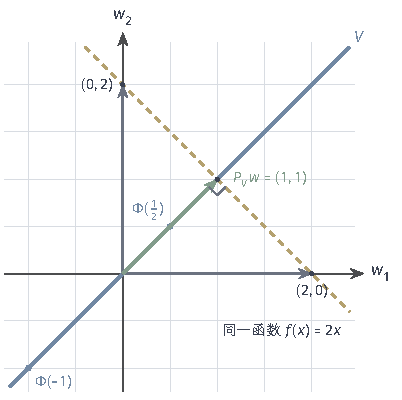
\includegraphics[width=68.1mm]{figures/02-abstract-mathematics/03-function-spaces/tikz/c5-visible-parameters/figure.pdf}
  \caption{冗余特征$\Phi(x)=(x,x)$的参数平面。特征值$\Phi(x)$都落在蓝色直线$V$上；黄色虚线上的参数都给出同一函数$f(x)=2x$。其中与$V$相交的$P_Vw=(1,1)$长度最短，为$\sqrt2$，这就是$\|f\|_{H_K}$；$(2,0)$与$(0,2)$长度为$2$，多出的部分来自对函数没有影响的$V^\perp$方向。}
  \label{fig:rkhs-visible-parameters}
\end{figure}

\subsection{核的运算}
\label{sec:rkhs-kernel-operations}

特征映射适合验证可以写成内积的核。更多的核是由几种基本核经过加法、乘法和换输入等运算得到的；只要这些运算保持半正定性，就不必为每个新核重新寻找特征映射。

\paragraph{保持半正定性的运算}

\begin{theorem}[核的运算]
\label{thm:rkhs-kernel-operations}
设$K_1,K_2$是非空集合$X$上的半正定核。则下列函数都是半正定核：
\begin{enumerate}
\item 非负线性组合$\alpha K_1+\beta K_2$，其中$\alpha,\beta\ge0$；
\item 逐点乘积$K_1(x,z)K_2(x,z)$；
\item 换输入：对任意集合$Y$和映射$\varphi:Y\to X$，$Y$上的$K_1(\varphi(y),\varphi(y'))$；
\item 函数缩放：对任意$g:X\to\mathbb R$，$g(x)g(z)K_1(x,z)$；
\item 逐点极限：若半正定核$K^{(n)}$在每个$(x,z)$处收敛到$K(x,z)$，则$K$半正定。
\end{enumerate}
\end{theorem}

\begin{proof}
固定点组$x_1,\ldots,x_n$与系数向量$\bm c$，记$\bm G_1,\bm G_2$为两个核的Gram矩阵。第1条：$\bm c^{\top}(\alpha\bm G_1+\beta\bm G_2)\bm c=\alpha\bm c^{\top}\bm G_1\bm c+\beta\bm c^{\top}\bm G_2\bm c\ge0$；用特征映射表达，把$\sqrt\alpha\,\Phi_1(x)$与$\sqrt\beta\,\Phi_2(x)$拼接成直和空间中的一个向量即可。

第2条：乘积核的Gram矩阵是逐元素乘积$\bm G_1\odot\bm G_2$。半正定矩阵$\bm G_2$可分解为$\bm G_2=\bm B\bm B^{\top}$（例如由谱分解取$\bm B=\bm U\bm\Lambda^{1/2}$），记$\bm b_k$为$\bm B$的第$k$列，则
\[
\bm c^{\top}(\bm G_1\odot\bm G_2)\bm c
=\sum_{i,j}c_ic_j(\bm G_1)_{i,j}\sum_k\bm B_{i,k}\bm B_{j,k}
=\sum_k(\bm c\odot\bm b_k)^{\top}\bm G_1(\bm c\odot\bm b_k)\ge0 .
\]
这就是Schur乘积定理。若两个核分别有有限维特征映射，乘积核的特征映射是张量积$\Phi_1(x)\otimes\Phi_2(x)$，因为$\langle u\otimes v,u'\otimes v'\rangle=\langle u,u'\rangle\langle v,v'\rangle$。

第3条：点组$y_1,\ldots,y_n$上的Gram矩阵就是点组$\varphi(y_1),\ldots,\varphi(y_n)$上$K_1$的Gram矩阵（允许点重复）。第4条：二次型等于$(\bm c\odot\bm g)^{\top}\bm G_1(\bm c\odot\bm g)$，其中$\bm g=(g(x_1),\ldots,g(x_n))$。第5条：每个二次型$\bm c^{\top}\bm G^{(n)}\bm c$非负，有限和的极限仍非负。
\end{proof}

逐元素乘积的半正定性和张量积的内积公式都是有限维线性代数中的结论，可参考\BookChapterRef{chap:normed-inner-product-spaces}{卷一《数学准备：基础数学》“赋范空间与内积空间”章中的Gram矩阵与Schur乘积}及\BookChapterRef{chap:linear-operations}{卷一“向量、矩阵与张量的运算”章中的张量积}。这里只用到它们在有限点组上的形式。

\paragraph{线性核、多项式核与高斯核}

由这几条规则可以验证常用的核。在$\mathbb R^d$上，\term{线性核}$K(\bm x,\bm z)=\bm x^{\top}\bm z$以$\Phi(\bm x)=\bm x$为特征映射。常数$c\ge0$是以$\sqrt c$为特征的核，于是$c+\bm x^{\top}\bm z$半正定（第1条），它的$p$次幂即\term{多项式核}$(c+\bm x^{\top}\bm z)^p$也半正定（第2条反复使用）。

\term{高斯核}（Gaussian kernel）$K_\sigma(\bm x,\bm z)=\exp\bigl(-\|\bm x-\bm z\|_2^2/(2\sigma^2)\bigr)$分三步验证。先把指数中的平方展开：
\[
\exp\Bigl(-\frac{\|\bm x-\bm z\|_2^2}{2\sigma^2}\Bigr)
=g(\bm x)\,g(\bm z)\,\exp\Bigl(\frac{\bm x^{\top}\bm z}{\sigma^2}\Bigr),\qquad
g(\bm x)=\exp\Bigl(-\frac{\|\bm x\|_2^2}{2\sigma^2}\Bigr).
\]
再看中间的因子：对每个$N$，部分和$\sum_{k=0}^N(\bm x^{\top}\bm z)^k/(k!\,\sigma^{2k})$是线性核的幂的非负组合，因而半正定；指数级数在每一点收敛，由第5条，极限$\exp(\bm x^{\top}\bm z/\sigma^2)$半正定。最后由第4条乘上$g(\bm x)g(\bm z)$。

\paragraph{运算在核截面上的效果}

核运算直接作用在核截面上：和核的截面是两个截面之和，乘积核的截面是两个截面之积。图~\ref{fig:rkhs-kernel-operations}在$x=0.4$处比较仿射核与高斯核（$\sigma=0.3$）。和核的截面在仿射趋势上叠加了一个局部隆起；乘积核的截面仍集中在$x$附近，但被仿射因子$1+0.4t$拉得右高左低。这说明乘积核所对应空间中的函数同时带有两种核的特点：局部性来自高斯因子，倾斜来自仿射因子。

\begin{figure}[!htb]
  \centering
  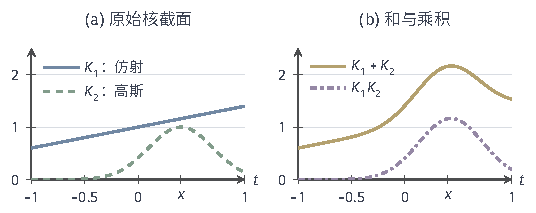
\includegraphics[width=90.7mm]{figures/02-abstract-mathematics/03-function-spaces/tikz/c5-kernel-operations/figure.pdf}
  \caption{核运算在核截面上的效果，固定$x=0.4$，$t\in[-1,1]$。(a)~仿射核截面$1+0.4t$与高斯核截面（$\sigma=0.3$）；(b)~两者之和与逐点乘积。和核的截面是两个截面相加，乘积核的截面是两个截面相乘，仍保持以$x$为中心的局部形状。}
  \label{fig:rkhs-kernel-operations}
\end{figure}

\paragraph{半正定性给不出的结论}

上面的规则只涉及非负组合、乘积与极限，减法不在其中。两个半正定核之差一般不是半正定核：仿射核减去常数核$2$得到$xz-1$，它在$x=z=0$处的对角值为$-1$，而半正定核的对角值$K(x,x)$必须非负。

半正定性也不包含更强的性质。二次多项式核$(1+xz)^2$在$\mathbb R$上半正定，但由特征映射$(1,\sqrt2x,x^2)$与定理~\ref{thm:rkhs-feature-space}，它的RKHS就是至多二次的多项式全体，任意四个点上的Gram矩阵都奇异，所以它不是严格正定核。这个三维空间在$C[-1,1]$中是闭的，不能一致逼近$|x|$这样的连续函数。高斯核既严格正定，又能用有限核和逼近紧区间上的任意连续函数，但后一性质需要第~\ref{sec:apx-kernel-sections}节专门的稠密性论证，不能从半正定性推出。

% 第5章第3节：有限观测与核表示（观测确定的函数子空间、有限中心的投影表示）。

\section{有限观测与核表示}
\label{sec:rkhs-finite-observations}

回到章首的传感器问题：我们只在有限个位置读到函数值。第~\ref{sec:lfo-finite-observations}节在有限维候选空间中讨论过一般线性观测，把每条读取规则写成观测矩阵的一行；那里的关键条件是观测在候选空间上满列秩。RKHS通常是无限维的，有限个读数不可能确定整个函数，问题于是变成：读数究竟确定了函数的哪一部分？由再生性质，每个点值读取都是与一个核截面的内积，所以答案可以用核截面张成的子空间和正交投影完整写出。本节先说明读数看见与看不见的方向，再把投影写成核矩阵方程，并讨论读数之外的误差和由观测点得到的有限维核。

\subsection{观测确定的函数子空间}
\label{sec:rkhs-observed-subspace}

固定RKHS $H$及其再生核$K$，取互异的观测位置$Z=\{x_1,\ldots,x_n\}\subseteq X$。对$f\in H$，读数向量是$\bm b=(f(x_1),\ldots,f(x_n))^{\top}$。

\paragraph{观测子空间与余项}

由再生性质，$f(x_i)=\langle f,K_{x_i}\rangle$，读数只与$f$在核截面$K_{x_1},\ldots,K_{x_n}$上的内积有关。令
\[
M_Z=\operatorname{span}\{K_{x_1},\ldots,K_{x_n}\},
\]
它是有限维子空间，因而是闭的。记$P=P_{M_Z}$为到$M_Z$的正交投影（第~\ref{sec:fs-projection}节），把$f$分解为$f=Pf+r$，其中$r\perp M_Z$。余项与每个$K_{x_i}$正交，正是说$r(x_i)=\langle r,K_{x_i}\rangle=0$。

\begin{theorem}[观测子空间]
\label{thm:rkhs-observed-subspace}
在上述记号下，$M_Z^\perp=\{g\in H:g(x_1)=\cdots=g(x_n)=0\}$。对$f,g\in H$，下列三条等价：$f$与$g$在$Z$上读数相同；$f-g\in M_Z^\perp$；$Pf=Pg$。
\end{theorem}

\begin{proof}
$g\perp M_Z$当且仅当$g$与每个$K_{x_i}$正交，即$g(x_i)=0$对每个$i$成立，这给出第一个等式。$f$与$g$读数相同，当且仅当$f-g$在每个$x_i$处取零，即$f-g\in M_Z^\perp$。由$H=M_Z\oplus M_Z^\perp$，$f-g\in M_Z^\perp$当且仅当$P(f-g)=0$。
\end{proof}

所以有限个点值恰好确定投影$Pf$，余项$r$则完全看不见：它在每个观测点取零，不论多大都不会改变任何读数。图~\ref{fig:rkhs-observation-residual}给出一个具体例子。取$[0,1]$上$\sigma=0.15$的高斯核，目标$f=K_{0.2}-0.8K_{0.5}+0.9K_{0.8}$，观测点$x_1,\ldots,x_4=0.1,0.35,0.6,0.9$。投影$Pf$与$f$在四个观测点重合，在观测点之间却可以明显不同；余项$r=f-Pf$在观测点处为零，在两点之间的振幅达到$0.41$。按范数计算，$\|f\|_H^2=2.039$，其中$\|Pf\|_H^2=1.210$被观测看见，其余$\|r\|_H^2=0.829$完全看不见。

\begin{figure}[!htb]
  \centering
  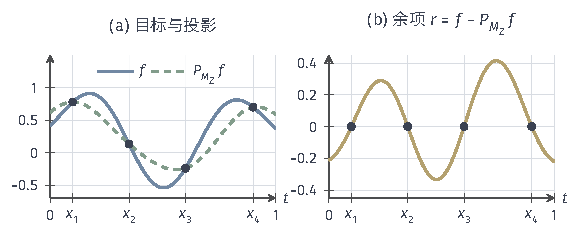
\includegraphics[width=97.9mm]{figures/02-abstract-mathematics/03-function-spaces/tikz/c5-observation-residual/figure.pdf}
  \caption{高斯核（$\sigma=0.15$）空间中的观测投影。(a)~目标$f=K_{0.2}-0.8K_{0.5}+0.9K_{0.8}$（实线）与它在$M_Z=\operatorname{span}\{K_{x_1},\ldots,K_{x_4}\}$上的投影（虚线），观测点$x_i=0.1,0.35,0.6,0.9$处两者取值相同（黑点）；(b)~余项$r=f-P_{M_Z}f$在每个观测点为零。读数只确定投影，余项对读数没有任何影响。}
  \label{fig:rkhs-observation-residual}
\end{figure}

\paragraph{Gram矩阵、读数与范数}

$M_Z$中的元素都能写成$g=\sum_ja_jK_{x_j}$，它的读数和范数都可以用Gram矩阵$\bm G_{i,j}=K(x_i,x_j)$计算：
\begin{equation}
\begin{gathered}
g(x_i)=\sum_ja_jK(x_i,x_j)=(\bm G\bm a)_i,\qquad
\|g\|_H^2=\bm a^{\top}\bm G\bm a,\\
\Bigl\langle\sum_ja_jK_{x_j},\sum_jc_jK_{x_j}\Bigr\rangle_H=\bm a^{\top}\bm G\bm c .
\end{gathered}
\label{eq:rkhs-gram-calculus}
\end{equation}
因此在$M_Z$内部，函数的全部计算都化为$n$维向量与$n\times n$矩阵的计算。注意$\bm a^{\top}\bm G\bm a$才是函数的范数平方，系数向量的欧氏长度$\|\bm a\|_2$一般与函数范数无关。

\paragraph{系数的不唯一与函数的不唯一}

有限观测下有两种不同的不唯一，它们来自不同的地方。第一种是系数的不唯一：两个系数向量$\bm a,\bm a'$给出同一个函数，当且仅当$\bigl\|\sum_j(a_j-a_j')K_{x_j}\bigr\|^2=(\bm a-\bm a')^{\top}\bm G(\bm a-\bm a')=0$，对半正定矩阵这等价于$\bm G(\bm a-\bm a')=\bm 0$。所以系数的冗余由$\ker\bm G$描述，它只是同一函数的不同写法。第二种是函数的不唯一：读数相同的函数可以相差$M_Z^\perp$中的任意元素，它们是真正不同的函数。

两个例子说明这两种情况互不决定。在仿射空间$H_{\mathrm{aff}}$中取$Z=\{-1,0,1\}$，第~\ref{sec:rkhs-kernel-properties}节已算出$\ker\bm G=\operatorname{span}\{(1,-2,1)\}$，系数不唯一；但三个核截面已经张成整个二维空间，$M_Z^\perp=\{0\}$，读数唯一确定函数。在$H_{\min}$中取$Z=\{1/3,2/3,1\}$，Gram矩阵
\[
\bm G=\frac13\begin{bmatrix}1&1&1\\1&2&2\\1&2&3\end{bmatrix},\qquad
\det\bm G=\frac1{27},
\]
可逆，系数唯一；但$M_Z^\perp$由在这三点取零的$H_{\min}$函数组成，是无限维的，读数远不能确定函数。若$K$严格正定，互异点上的Gram矩阵总可逆，第一种不唯一不会出现，第二种在无限维空间中却总是存在。

\subsection{有限中心的投影表示}
\label{sec:rkhs-center-projection}

上一小节说明读数确定$Pf$。现在把$Pf$实际算出来，即求出它在核截面$K_{x_1},\ldots,K_{x_n}$上的系数；这些观测位置在表示中充当中心。

\paragraph{正交条件与核矩阵方程}

设$Pf=\sum_ja_jK_{x_j}$。投影由正交条件$\langle f-Pf,K_{x_i}\rangle=0$（$i=1,\ldots,n$）刻画，由再生性质，它就是$(Pf)(x_i)=f(x_i)$，再由式~\eqref{eq:rkhs-gram-calculus}，
\begin{equation}
\bm G\bm a=\bm b,\qquad \bm b_i=f(x_i).
\label{eq:rkhs-center-equation}
\end{equation}
投影的正交条件与“在观测点插值”在这里是同一组方程。

\begin{theorem}[有限中心的投影]
\label{thm:rkhs-center-projection}
设$\bm b$是某个$f\in H$在$Z$上的读数。则：
\begin{enumerate}
\item 方程~\eqref{eq:rkhs-center-equation}有解，任意一个解$\bm a$都给出同一个函数$\sum_ja_jK_{x_j}=Pf$；
\item $Pf$是$M_Z$中唯一在$Z$上取读数$\bm b$的函数，也是$H$中所有满足$g(x_i)=\bm b_i$的函数$g$里范数最小的一个，且$\|Pf\|_H^2=\bm b^{\top}\bm a=\bm b^{\top}\bm G^{\dagger}\bm b$。
\end{enumerate}
\end{theorem}

\begin{proof}
$Pf\in M_Z$，可写成$\sum_ja_j^*K_{x_j}$，而$Pf$与$f$读数相同，所以$\bm G\bm a^*=\bm b$，方程相容。若$\bm G\bm a=\bm b=\bm G\bm a^*$，则$\bm a-\bm a^*\in\ker\bm G$，上一小节说明两组系数给出同一函数。对第2条，$M_Z$中两个读数相同的函数之差属于$M_Z\cap M_Z^\perp=\{0\}$。若$g\in H$满足$g(x_i)=\bm b_i$，则$g-Pf$在$Z$上取零，属于$M_Z^\perp$，勾股定理给出$\|g\|^2=\|Pf\|^2+\|g-Pf\|^2\ge\|Pf\|^2$。最后，$\|Pf\|^2=\bm a^{\top}\bm G\bm a=\bm a^{\top}\bm b$；取$\bm a=\bm G^{\dagger}\bm b$即得最后一个表达式。
\end{proof}

第1条区分了投影的唯一性与系数的唯一性。$\bm G$奇异时，可以用伪逆$\bm G^{\dagger}$从相容方程的全部解中选出欧氏长度最小的系数，这一性质可参考\BookChapterRef{chap:linear-equations-and-optimization}{卷一《数学准备：基础数学》“线性方程与矩阵方程”章中的伪逆与最小范数解}。但无论选哪一组系数，得到的函数都是同一个$Pf$；系数长度最小与函数范数最小是两回事，后者由第2条保证，与系数怎样选取无关。

\paragraph{最小值核的投影是折线插值}

在$H_{\min}$中，中心投影有一个直观的形式。取$Z=\{1/3,2/3,1\}$，$M_Z$由核截面$\min(\cdot,1/3)$、$\min(\cdot,2/3)$、$\min(\cdot,1)$张成，即在$1/3,2/3$处可以转折、左端为零的连续折线。由定理~\ref{thm:rkhs-center-projection}，$Pf$就是过原点和三个观测点的折线插值。以$f(x)=4x(1-x)$为例，读数为$\bm b=(8/9,8/9,0)$。折线在三段上的斜率依次为$8/3$、$0$、$-8/3$；而$\sum_ja_j\min(t,x_j)$在三段上的斜率依次为$a_1+a_2+a_3$、$a_2+a_3$、$a_3$，于是$\bm a=(8/3,8/3,-8/3)$。代回检验$\bm G\bm a=\bm b$：第一行$\tfrac13\cdot\tfrac83=\tfrac89$，第二行$\tfrac13\cdot\tfrac83+\tfrac23\cdot\tfrac83-\tfrac23\cdot\tfrac83=\tfrac89$，第三行$\tfrac89+\tfrac{16}9-\tfrac{24}9=0$。第~\ref{sec:rkhs-finite-features}节还会用到这个例子。

\paragraph{读数之外的误差}

投影在观测点上没有误差，那么在观测点之间误差有多大？由再生性质与$r\perp M_Z$，对任意$x\in X$，
\[
f(x)-(Pf)(x)=r(x)=\langle r,K_x\rangle=\langle r,K_x-PK_x\rangle ,
\]
第三个等号是因为$PK_x\in M_Z$与$r$正交。由Cauchy--Schwarz不等式，
\begin{equation}
|f(x)-(Pf)(x)|\le P_Z(x)\,\|f-Pf\|_H\le P_Z(x)\,\|f\|_H,
\label{eq:rkhs-power-bound}
\end{equation}
其中$P_Z(x)=\|K_x-PK_x\|_H$。
称$P_Z$为观测点组$Z$的\term{核插值幂函数}（power function）。它只依赖于核与观测位置，不依赖于目标函数：$P_Z(x)$是核截面$K_x$中不能被观测子空间表示的部分的长度。

$P_Z$可以用核矩阵算出。$PK_x$本身是一个投影，它的读数就是$K_x$的读数$\bm k_Z(x)=(K(x_1,x),\ldots,K(x_n,x))^{\top}$，由定理~\ref{thm:rkhs-center-projection}，$\|PK_x\|^2=\bm k_Z(x)^{\top}\bm G^{\dagger}\bm k_Z(x)$，再由勾股定理，
\begin{equation}
P_Z(x)^2=K(x,x)-\bm k_Z(x)^{\top}\bm G^{\dagger}\bm k_Z(x).
\label{eq:rkhs-power-function}
\end{equation}
在观测点$x=x_i$处，$K_{x_i}\in M_Z$，所以$P_Z(x_i)=0$。图~\ref{fig:rkhs-power-function}画出前一个高斯核例子的幂函数：它在四个观测点处为零，在相邻观测点之间隆起；间隔越大或离观测点越远，隆起越高，最大值约为$0.59$，出现在区间端点附近和$x_3,x_4$之间。同一图中，余项$|r(x)|$始终位于上界$P_Z(x)\|r\|_H$之下（这里$\|r\|_H=0.911$）。对最小值核，$K_x-PK_x$是$\min(\cdot,x)$减去它的折线插值，在$x$所在的小区间$[x_{k-1},x_k]$上是一个三角形，直接计算导数的平方积分得$P_Z(x)^2=(x-x_{k-1})(x_k-x)/(x_k-x_{k-1})$（约定$x_0=0$）。

\begin{figure}[!htb]
  \centering
  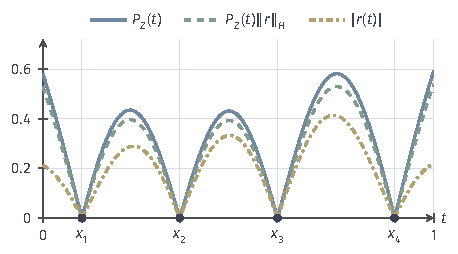
\includegraphics[width=77.5mm]{figures/02-abstract-mathematics/03-function-spaces/tikz/c5-power-function/figure.pdf}
  \caption{高斯核（$\sigma=0.15$）、观测点$x_i=0.1,0.35,0.6,0.9$的核插值幂函数$P_Z(t)=\|K_t-PK_t\|_H$（实线），以及图~\ref{fig:rkhs-observation-residual}中余项的绝对值$|r(t)|$（点划线）与上界$P_Z(t)\|r\|_H$（虚线，$\|r\|_H=0.911$）。幂函数在观测点处为零，只依赖于核与观测位置；余项总在上界之下。}
  \label{fig:rkhs-power-function}
\end{figure}

\paragraph{观测子空间自身的再生核}

前面处理的是一个给定函数的投影。换一个角度，观测子空间$M_Z$连同$H$的内积本身也是一个RKHS：对$g\in M_Z$，$g(x)=\langle g,K_x\rangle=\langle g,PK_x\rangle$，所以它的核截面是$PK_x$，再生核为
\begin{equation}
K_Z(x,z)=\langle PK_z,PK_x\rangle_H=\bm k_Z(x)^{\top}\bm G^{\dagger}\bm k_Z(z).
\label{eq:rkhs-projected-kernel}
\end{equation}
第二个等号用了$PK_x=\sum_jc_j(x)K_{x_j}$、$\bm c(x)=\bm G^{\dagger}\bm k_Z(x)$，以及式~\eqref{eq:rkhs-gram-calculus}和$\bm G^{\dagger}\bm G\bm G^{\dagger}=\bm G^{\dagger}$。同理，余下的$K-K_Z$是$M_Z^\perp$的再生核，因而也半正定，它的对角值就是$P_Z(x)^2$。

式~\eqref{eq:rkhs-projected-kernel}可以写成有限特征的内积。设$\bm G=\bm U\bm\Lambda\bm U^{\top}$是谱分解，$r$个正特征值组成$\bm\Lambda_r$，相应的特征向量组成$\bm U_r$。令
\[
\Phi_Z(x)=\bm\Lambda_r^{-1/2}\bm U_r^{\top}\bm k_Z(x)\in\mathbb R^r ,
\]
则$\Phi_Z(x)^{\top}\Phi_Z(z)=\bm k_Z(x)^{\top}\bm U_r\bm\Lambda_r^{-1}\bm U_r^{\top}\bm k_Z(z)=K_Z(x,z)$。$\Phi_Z$的第$k$个分量是函数$e_k=\lambda_k^{-1/2}\sum_j\bm U_{j,k}K_{x_j}$在$x$处的值，这些$e_k$构成$M_Z$的标准正交基：由式~\eqref{eq:rkhs-gram-calculus}，$\langle e_k,e_l\rangle=\lambda_k^{-1/2}\lambda_l^{-1/2}\bm u_k^{\top}\bm G\bm u_l=\delta_{k,l}$。

这里要分清两种近似。$Pf$近似的是一个给定的函数，误差取决于该函数的余项；$K_Z$近似的是核本身，它同时为$M_Z$中的所有函数提供再生关系，误差$K-K_Z$不涉及任何目标函数。式~\eqref{eq:rkhs-power-bound}把两者联系起来：给定函数的逐点误差不超过核误差的对角平方根乘以该函数的余项范数。中心应当怎样选取、读数带有噪声时采用什么拟合目标与惩罚、所得问题的解是否存在，都需要另外加入目标与观测模型；以核矩阵为工具的正则化回归可参考\BookChapterRef{chap:regression}{卷七《模型：经典模型》“回归”章中的核岭回归}，按样本抽取中心的低秩近似可参考\BookChapterRef{chap:dimensionality-reduction}{卷七“降维”章中的Nyström近似}。

% 第5章第4节：核的谱表示与有限特征（核积分算子与Mercer展开、核范数与谱系数、有限谱特征）。

\section{核的谱表示与有限特征}
\label{sec:rkhs-spectral}

到目前为止，核空间的全部结构都只由核决定，没有用到测度。本节固定核后再在输入集上加入一个测度，用核作积分核得到积分算子，从而把第~\ref{chap:operator-spectra-equations}章的紧自伴谱理论用到核上。要回答三个问题：积分算子的特征函数能否组成核本身的逐点展开；核范数在这些正交坐标下是什么形式；只保留前几个谱方向时，被控制的是核的误差还是某个给定函数的误差。

全节使用下面的条件：$X$是紧度量空间，$K$是$X\times X$上连续的半正定核，$\mu$是$X$上的有限正Borel测度，且具有\term{全支撑}（full support），即$X$的每个非空开集测度为正。记$M^2=\max_{x\in X}K(x,x)$。

\subsection{核积分算子与Mercer展开}
\label{sec:rkhs-mercer}
\label{subsubsec:compact-spectrum-mercer}

\paragraph{核积分算子}

在上述条件下定义\term{核积分算子}（kernel integral operator）
\[
(T_Kf)(x)=\int_XK(x,z)f(z)\,\mathrm d\mu(z),\qquad f\in L^2(\mu).
\]
$K$连续且$X$紧，所以$K$有界，又$\mu$有限，于是$K\in L^2(\mu\otimes\mu)$。由第~\ref{sec:ose-hilbert-schmidt}节，$T_K$是$L^2(\mu)$上的紧算子；由$K$对称及第~\ref{sec:ose-kernel-symmetry}节，$T_K$自伴。第~\ref{sec:ose-kernels}节已经强调，核公式只有连同测度才确定一个算子；这里的测度正是在核之外新加入的结构。

$T_K$的像比$L^2$等价类好得多：对任意$g\in L^2(\mu)$，$T_Kg$是处处有定义的连续函数。事实上，由Cauchy--Schwarz不等式，
\[
\begin{aligned}
|(T_Kg)(x)-(T_Kg)(x')|
&\le\Bigl(\int_X|K(x,z)-K(x',z)|^2\,\mathrm d\mu(z)\Bigr)^{1/2}\|g\|_{L^2}\\
&\le\mu(X)^{1/2}\sup_{z\in X}|K(x,z)-K(x',z)|\,\|g\|_{L^2},
\end{aligned}
\]
而$K$在紧集$X\times X$上一致连续，右端随$x'\to x$趋于零。

\paragraph{积分算子的正性}

第~\ref{sec:ose-kernel-symmetry}节指出，核的对称性只给出自伴，不给出$\langle T_Kf,f\rangle\ge0$。这里的正性来自核的半正定性，但两者的联系需要一个逼近论证：半正定性只涉及有限点组，积分则是连续的累计。

\begin{lemma}[半正定连续核给出正算子]
\label{lem:rkhs-positive-operator}
在本节条件下，对一切$f\in L^2(\mu)$，$\langle T_Kf,f\rangle_{L^2}=\iint K(x,z)f(x)f(z)\,\mathrm d\mu(x)\,\mathrm d\mu(z)\ge0$。
\end{lemma}

\begin{proof}
先设$f$连续。给定$\varepsilon>0$，函数$(x,z)\mapsto K(x,z)f(x)f(z)$在紧集上一致连续，取$\delta>0$使两点距离小于$\delta$时它的变化小于$\varepsilon$。用有限个半径$\delta/2$的开球覆盖$X$，再把它们依次去掉重叠部分，得到$X$的有限Borel划分$A_1,\ldots,A_N$，每块直径小于$\delta$；在每块中任取一点$x_i$。在$A_i\times A_j$上用$K(x_i,x_j)f(x_i)f(x_j)$代替被积函数，误差不超过$\varepsilon$，所以
\[
\Bigl|\langle T_Kf,f\rangle-\sum_{i,j}K(x_i,x_j)c_ic_j\Bigr|\le\varepsilon\,\mu(X)^2,\qquad c_i=f(x_i)\mu(A_i).
\]
中间的和是点组$x_1,\ldots,x_N$上Gram矩阵的二次型，非负；令$\varepsilon\to0$即得$\langle T_Kf,f\rangle\ge0$。对一般的$f\in L^2(\mu)$，连续函数在$L^2(\mu)$中稠密（第~\ref{sec:fs-density-separability}节），而$f\mapsto\langle T_Kf,f\rangle$在$L^2$中连续，非负性保持到极限。
\end{proof}

\paragraph{特征函数的连续代表}

于是$T_K$是$L^2(\mu)$上的紧、自伴、正算子，第~\ref{sec:ose-spectral-theorem}节的谱定理给出：非零特征值都是正数，至多可数，按重数重复排列为$\lambda_1\ge\lambda_2\ge\cdots>0$，只能在零处聚集；相应的特征函数$\psi_j$构成$(\ker T_K)^\perp$的标准正交基。

特征函数起初只是$L^2$等价类。若$T_K\psi=\lambda\psi$且$\lambda>0$，则$\psi=\lambda^{-1}T_K\psi$几乎处处成立，右端是连续函数，所以$\psi$有连续代表，以下总取这个代表。全支撑保证这个代表唯一：两个连续函数若几乎处处相等，使它们不相等的点组成开集，测度为零，由全支撑只能是空集。若$\mu$没有全支撑，例如$X=[0,1]$而$\mu$只是$[0,1/2]$上的Lebesgue测度，那么在$[1/2,1]$上任意改动的函数仍是同一个$L^2$元素，$L^2$坐标就无法确定函数在测度支撑之外的取值。

\paragraph{Mercer定理}

谱定理给出的是算子作用的展开$T_Kf=\sum_j\lambda_j\langle f,\psi_j\rangle\psi_j$，它在$L^2$范数下成立。对核本身，我们希望得到逐点甚至一致的展开，这正是\term{Mercer定理}（Mercer theorem）的内容\scite{mercer1909functions}。

\begin{theorem}[Mercer定理]
\label{thm:rkhs-mercer}
设$X$是紧度量空间，$K$是$X\times X$上连续的半正定核，$\mu$是$X$上全支撑的有限正Borel测度。设$\lambda_j>0$与连续的$\psi_j$是$T_K$的正特征值与$L^2(\mu)$标准正交特征函数。则
\begin{equation}
K(x,z)=\sum_j\lambda_j\psi_j(x)\psi_j(z)\qquad(x,z\in X),
\label{eq:rkhs-mercer}
\end{equation}
级数在$X\times X$上绝对且一致收敛；并且$\sum_j\lambda_j=\int_XK(x,x)\,\mathrm d\mu(x)<\infty$。
\end{theorem}

\begin{proof}[补充阅读：证明思路]
第一步，对角线上的部分和有界。令
\[
K^{(m)}(x,z)=K(x,z)-\sum_{j\le m}\lambda_j\psi_j(x)\psi_j(z),
\]
它连续。由谱展开，它对应的积分算子$T^{(m)}$满足
\[
\langle T^{(m)}f,f\rangle=\sum_{j>m}\lambda_j\langle f,\psi_j\rangle^2\ge0 .
\]若$K^{(m)}(x_0,x_0)<0$，由连续性存在$x_0$的开邻域$U$使$K^{(m)}<0$在$U\times U$上成立，取$f=\mathbf 1_U$，全支撑给出$\mu(U)>0$，于是$\langle T^{(m)}f,f\rangle<0$，矛盾。所以$\sum_{j\le m}\lambda_j\psi_j(x)^2\le K(x,x)\le M^2$对一切$m$与$x$成立。

第二步，固定$x$识别极限。由Cauchy--Schwarz不等式与第一步，
\[
\sum_{j=p}^q\lambda_j|\psi_j(x)\psi_j(z)|\le\Bigl(\sum_{j=p}^q\lambda_j\psi_j(x)^2\Bigr)^{1/2}M ,
\]
而第一步说明右端括号中的级数收敛，所以对固定的$x$，级数$S(x,z)=\sum_j\lambda_j\psi_j(x)\psi_j(z)$关于$z$一致收敛，$S(x,\cdot)$连续。另一方面，$\langle K(x,\cdot),\psi_j\rangle_{L^2}=(T_K\psi_j)(x)=\lambda_j\psi_j(x)$，所以连续函数$h=K(x,\cdot)-S(x,\cdot)$与每个$\psi_j$正交，属于$\ker T_K$；由于$T_Kh$连续且几乎处处为零，它处处为零，特别地$\int K(x,z)h(z)\,\mathrm d\mu(z)=0$。又$\int S(x,z)h(z)\,\mathrm d\mu(z)=\sum_j\lambda_j\psi_j(x)\langle\psi_j,h\rangle=0$，两式相减得$\int h^2\,\mathrm d\mu=0$。由全支撑与连续性，$h\equiv0$，即$K(x,z)=S(x,z)$。

第三步，一致收敛。在对角线上，连续函数$R_m(x)=K(x,x)-\sum_{j\le m}\lambda_j\psi_j(x)^2$随$m$单调下降并逐点趋于零。对任意$\varepsilon>0$，闭集$\{R_m\ge\varepsilon\}$随$m$递减且交为空集，由$X$的紧性，其中某一个已是空集，所以$R_m\to0$一致成立（这就是Dini定理）。再由第二步的Cauchy--Schwarz估计，$\sum_{j>m}\lambda_j|\psi_j(x)\psi_j(z)|\le\sqrt{R_m(x)R_m(z)}\le\max R_m$，得到$X\times X$上的绝对一致收敛。最后对对角线逐项积分（一致收敛且$\mu$有限），$\int K(x,x)\,\mathrm d\mu=\sum_j\lambda_j\int\psi_j^2\,\mathrm d\mu=\sum_j\lambda_j$。
\end{proof}

正特征值之和有限，说明$T_K$是\term{迹类算子}（trace-class operator）。比较两种展开：一般的紧自伴谱定理只说算子作用在$L^2$范数下展开，展开中的特征函数只是等价类；Mercer定理在核的连续性、半正定性与测度全支撑的条件下，给出核本身的逐点、一致展开，其中每个$\psi_j$都取连续代表。零特征值方向不出现在展开~\eqref{eq:rkhs-mercer}中；任何形如“除以$\lambda_j$”的公式，都只能在正谱方向上使用。

\paragraph{仿射核的谱}

第~\ref{sec:ose-kernels}节在$X=[-1,1]$、$\mathrm d\mu(z)=\mathrm dz/2$下计算过仿射核$K(x,z)=1+xz$的积分算子：$T_K1=1$，$T_Kx=x/3$，与$1,x$都正交的函数被消去。于是正特征值为$\lambda_1=1$、$\lambda_2=1/3$，标准正交特征函数为$\psi_1=1$、$\psi_2=\sqrt3\,x$（$\int3x^2\,\mathrm d\mu=1$）。Mercer展开只有两项：
\[
\lambda_1\psi_1(x)\psi_1(z)+\lambda_2\psi_2(x)\psi_2(z)=1+\tfrac13\cdot3xz=1+xz ,
\]
迹为$1+\tfrac13=\int_{-1}^1(1+x^2)\,\tfrac{\mathrm dx}2=\tfrac43$。零空间是$L^2(\mu)$中与$1,x$正交的全部函数，例如$x^2-1/3$。它是无限维的，却不出现在核的展开中。

\paragraph{最小值核的谱}

最小值核给出无穷多个正特征值，而且可以精确算出。在$[0,1]$上取Lebesgue测度，
\[
(T_K\psi)(x)=\int_0^xz\psi(z)\,\mathrm dz+x\int_x^1\psi(z)\,\mathrm dz .
\]
对连续的$\psi$，右端可微两次：$(T_K\psi)'(x)=\int_x^1\psi(z)\,\mathrm dz$，$(T_K\psi)''=-\psi$；并且$(T_K\psi)(0)=0$、$(T_K\psi)'(1)=0$。所以$T_K\psi=\lambda\psi$（$\lambda>0$）等价于边值问题$\lambda\psi''=-\psi$、$\psi(0)=0$、$\psi'(1)=0$，其解为$\psi(x)=\sin(\omega x)$，$\omega=\lambda^{-1/2}$且$\cos\omega=0$。归一化后
\[
\lambda_j=\frac1{\omega_j^2},\qquad \psi_j(x)=\sqrt2\,\sin(\omega_jx),\qquad \omega_j=\Bigl(j-\frac12\Bigr)\pi,\quad j=1,2,\ldots
\]
同样的推导说明$T_K\psi=0$迫使$\psi=-(T_K\psi)''=0$，所以零空间是平凡的，这些$\psi_j$构成$L^2(0,1)$的标准正交基。迹的检验：$\sum_j\lambda_j=\sum_j\frac{4}{(2j-1)^2\pi^2}=\frac12=\int_0^1x\,\mathrm dx$。

图~\ref{fig:rkhs-mercer-spectrum}画出前三个特征函数，并比较三种核的特征值衰减。最小值核的特征值按$j^{-2}$衰减；$\sigma=0.5$的高斯核在$[-1,1]$、$\mathrm dz/2$下的特征值衰减得快得多，第$12$个已降到$5\times10^{-9}$量级（数值求积所得）；仿射核只有两个正特征值。核越光滑，积分算子越强烈地压低高频方向，这里只作观察，不作为一般定理使用。

\begin{figure}[!htb]
  \centering
  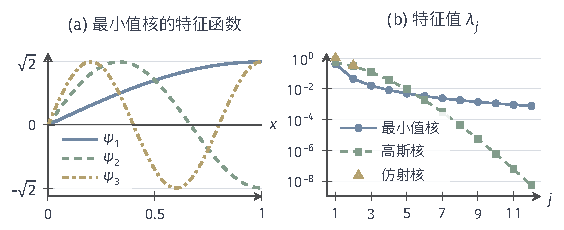
\includegraphics[width=95.5mm]{figures/02-abstract-mathematics/03-function-spaces/tikz/c5-mercer-spectrum/figure.pdf}
  \caption{Mercer特征函数与特征值衰减。(a)~最小值核在$[0,1]$、Lebesgue测度下的前三个特征函数$\psi_j=\sqrt2\sin((j-\frac12)\pi x)$，它们在$0$处为零、在$1$处导数为零；(b)~特征值（对数纵轴）：最小值核$\lambda_j=((j-\frac12)\pi)^{-2}$；高斯核（$\sigma=0.5$，$[-1,1]$，$\mathrm dz/2$）的特征值由40点Gauss--Legendre求积离散计算；仿射核只有$1$与$1/3$两个正特征值。}
  \label{fig:rkhs-mercer-spectrum}
\end{figure}

\subsection{核范数与谱系数}
\label{sec:rkhs-spectral-norm}

Mercer展开把核写成了特征映射$\Phi(x)=(\sqrt{\lambda_j}\psi_j(x))_j$的内积，这正好可以代入第~\ref{sec:rkhs-feature-maps}节的定理，读出核范数在谱坐标下的形式。

\paragraph{谱坐标下的核范数}

\begin{theorem}[核范数的谱表示]
\label{thm:rkhs-spectral-norm}
在定理~\ref{thm:rkhs-mercer}的条件下：
\begin{enumerate}
\item $\{\sqrt{\lambda_j}\,\psi_j\}$是$H_K$的标准正交基；
\item 函数$f:X\to\mathbb R$属于$H_K$，当且仅当存在实数列$(b_j)$满足$\sum_jb_j^2/\lambda_j<\infty$，且$f(x)=\sum_jb_j\psi_j(x)$对一切$x$成立。此时级数在$X$上绝对一致收敛，$b_j=\langle f,\psi_j\rangle_{L^2(\mu)}$，并且
\begin{equation}
\|f\|_{L^2(\mu)}^2=\sum_jb_j^2,\qquad \|f\|_{H_K}^2=\sum_j\frac{b_j^2}{\lambda_j}.
\label{eq:rkhs-two-norms}
\end{equation}
\end{enumerate}
\end{theorem}

\begin{proof}
令$\mathcal F=\ell^2$，$\Phi(x)=(\sqrt{\lambda_j}\psi_j(x))_j$。由定理~\ref{thm:rkhs-mercer}的第一步，$\|\Phi(x)\|^2=K(x,x)<\infty$；由Mercer展开，$\langle\Phi(x),\Phi(z)\rangle=K(x,z)$，所以$\Phi$是$K$的特征映射。先证可见子空间是整个$\ell^2$。设$w\in\ell^2$与每个$\Phi(x)$正交，即$\sum_jw_j\sqrt{\lambda_j}\psi_j(x)=0$对一切$x$成立。由于$\sqrt{\lambda_j}\le\sqrt{\lambda_1}$，系数$w_j\sqrt{\lambda_j}$平方可和，同一级数在$L^2(\mu)$中也收敛，其$L^2$极限与逐点极限几乎处处一致，因而为零；由$\psi_j$的标准正交性，$w_j\sqrt{\lambda_j}=0$，即$w=0$。

于是由定理~\ref{thm:rkhs-feature-space}，$w\mapsto f_w=\sum_jw_j\sqrt{\lambda_j}\psi_j$是从$\ell^2$到$H_K$的等距同构，单位向量$e_j$映为$\sqrt{\lambda_j}\psi_j$，这证明第1条。令$b_j=w_j\sqrt{\lambda_j}$，条件$w\in\ell^2$就是$\sum_jb_j^2/\lambda_j<\infty$，且$\|f_w\|_{H_K}^2=\sum_jw_j^2=\sum_jb_j^2/\lambda_j$。一致收敛来自
\[
\Bigl|\sum_{j>m}b_j\psi_j(x)\Bigr|\le\Bigl(\sum_{j>m}\frac{b_j^2}{\lambda_j}\Bigr)^{1/2}\Bigl(\sum_{j>m}\lambda_j\psi_j(x)^2\Bigr)^{1/2}\le M\Bigl(\sum_{j>m}\frac{b_j^2}{\lambda_j}\Bigr)^{1/2} .
\]
一致收敛的级数也在$L^2(\mu)$中收敛到同一函数，由标准正交性得$b_j=\langle f,\psi_j\rangle_{L^2}$与$\|f\|_{L^2}^2=\sum_jb_j^2$。
\end{proof}

\paragraph{两种范数的权重}

式~\eqref{eq:rkhs-two-norms}说明，同一组谱坐标$b_j$在两种范数中得到不同的权重：$L^2$范数对每个坐标一视同仁，核范数则把第$j$个坐标的平方放大$1/\lambda_j$倍。$L^2$中的单位方向$\psi_j$在$H_K$中的长度是$\lambda_j^{-1/2}$，$H_K$中真正的单位方向是$\sqrt{\lambda_j}\psi_j$。由于$\lambda_j\to0$，特征值小的方向在核范数中代价很高。

图~\ref{fig:rkhs-norm-weights}用最小值核说明这种差别。$f=\psi_1$与$g=\psi_1+0.1\psi_8$的图像几乎重合，$\|f-g\|_{L^2}=0.1$；但$\|f-g\|_{H_{\min}}=0.1\,\omega_8=0.1\times7.5\pi\approx2.36$，比$\|f\|_{H_{\min}}=\omega_1=\pi/2\approx1.57$还大。积分误差小并不意味着核范数误差小，核范数还计入了函数的振荡：对最小值核，$\|f\|_{H_{\min}}=\|f'\|_{L^2}$，$g$的高频小波纹带来很大的导数。

\begin{figure}[!htb]
  \centering
  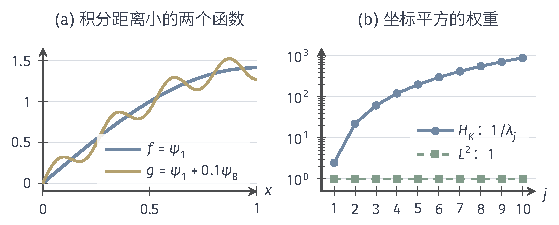
\includegraphics[width=94.6mm]{figures/02-abstract-mathematics/03-function-spaces/tikz/c5-norm-weights/figure.pdf}
  \caption{最小值核下两种范数的谱权重。(a)~$f=\psi_1$与$g=\psi_1+0.1\psi_8$，$\psi_j=\sqrt2\sin((j-\frac12)\pi x)$；两者的$L^2$距离为$0.1$，核范数距离却约为$2.36$。(b)~谱坐标平方在两种范数中的权重：$L^2$中恒为$1$，$H_K$中为$1/\lambda_j=((j-\frac12)\pi)^2$（对数纵轴），随$j$平方增长。}
  \label{fig:rkhs-norm-weights}
\end{figure}

\paragraph{哪些函数不在核空间中}

定理~\ref{thm:rkhs-spectral-norm}给出了$H_K$成员的两项要求：作为$L^2$元素，函数没有零谱分量；其谱坐标的加权平方和有限。两项要求可以分别不满足。在仿射核的例子中，$x^2=\tfrac13\psi_1+(x^2-\tfrac13)$含有零谱分量$x^2-\tfrac13$，所以不在$H_{\mathrm{aff}}$中，这一点也可以直接从$H_{\mathrm{aff}}$只含仿射函数看出。在最小值核的例子中零空间平凡，但常数函数$1$的谱坐标为$b_j=\int_0^1\sqrt2\sin(\omega_jx)\,\mathrm dx=\sqrt2/\omega_j$，于是$\sum_jb_j^2=\sum_j2/\omega_j^2=1=\|1\|_{L^2}^2$有限，而$\sum_jb_j^2/\lambda_j=\sum_j2$发散。常数$1$的谱展开在$L^2$中收敛，它却不属于$H_{\min}$，这与$H_{\min}$要求$f(0)=0$相符。

\paragraph{谱截断的两种尾和}

固定$f\in H_K$及其谱坐标$b_j$，令$f_m=\sum_{j\le m}b_j\psi_j$。由式~\eqref{eq:rkhs-two-norms}，
\begin{equation}
\|f-f_m\|_{L^2(\mu)}^2=\sum_{j>m}b_j^2\le\lambda_{m+1}\sum_{j>m}\frac{b_j^2}{\lambda_j}=\lambda_{m+1}\|f-f_m\|_{H_K}^2 ,
\label{eq:rkhs-tail-comparison}
\end{equation}
不等号用了$j>m$时$\lambda_j\le\lambda_{m+1}$。核范数尾和随$m\to\infty$趋于零，再由点值估计，
\[
|f(x)-f_m(x)|\le\sqrt{K(x,x)}\,\|f-f_m\|_{H_K}\le M\|f-f_m\|_{H_K},
\]
所以截断还一致收敛到$f$。逐点与一致控制来自核空间的点值有界性；一般的$L^2$正交展开没有这样的保证。式~\eqref{eq:rkhs-tail-comparison}还说明，对核范数不超过$R$的函数，$L^2$截断误差不超过$\sqrt{\lambda_{m+1}}R$，特征值衰减越快，这个统一的界越小。

以$H_{\min}$中的$f(x)=4x(1-x)$为例。它的谱坐标可以由分部积分算出：$b_j=4\sqrt2\bigl(2\omega_j^{-3}-(-1)^{j+1}\omega_j^{-2}\bigr)$，前三项约为$0.626,0.363,-0.068$；又$\|f\|_{L^2}^2=8/15$，$\|f\|_{H_{\min}}^2=\|f'\|_{L^2}^2=16/3$。取$m=3$，用总和减去前三项得$\|f-f_3\|_{L^2}\approx0.068$，$\|f-f_3\|_{H_{\min}}\approx1.07$。可以核对式~\eqref{eq:rkhs-tail-comparison}：$0.068^2\approx0.0046\le\lambda_4\times1.07^2\approx0.0083\times1.15\approx0.0095$。核范数尾和远大于$L^2$尾和，是因为$f'(1)=-4\ne0$而每个$\psi_j'(1)=0$，谱坐标只按$\omega_j^{-2}$衰减。

\paragraph{固定核而改变测度}

谱坐标依赖于测度，核范数却不依赖。仍取仿射核，把$[-1,1]$上的测度从$\mathrm dz/2$换成$\mathrm dz$，积分算子变为原来的两倍，特征值变为$2$与$2/3$，标准正交特征函数变为$1/\sqrt2$与$\sqrt{3/2}\,x$。对$f=a+bx$，新的谱坐标为$b_1=\sqrt2\,a$，$b_2=\int_{-1}^1(a+bx)\sqrt{3/2}\,x\,\mathrm dx=\sqrt{2/3}\,b$，于是
\[
\frac{b_1^2}{\lambda_1}+\frac{b_2^2}{\lambda_2}=\frac{2a^2}{2}+\frac{2b^2/3}{2/3}=a^2+b^2 ,
\]
与原来的核范数相同；而$L^2$范数平方从$a^2+b^2/3$变成了$2a^2+2b^2/3$。图~\ref{fig:rkhs-affine-norm-balls}在系数平面上画出三个单位球：核范数的单位球是圆，两个$L^2$单位球是形状不同的椭圆。这在一般情况下也成立：由定理~\ref{thm:rkhs-moore-aronszajn}，$H_K$的内积只由核决定；测度提供的是新的正交坐标和积分意义下的误差度量。

\begin{figure}[!htb]
  \centering
  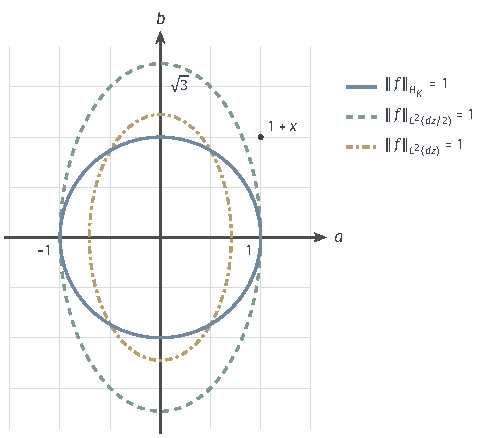
\includegraphics[width=82.4mm]{figures/02-abstract-mathematics/03-function-spaces/tikz/c5-affine-norm-balls/figure.pdf}
  \caption{仿射核$1+xz$在$[-1,1]$上，系数平面$(a,b)$（$f=a+bx$）中的三个单位球。实线圆是核范数单位球$a^2+b^2=1$，与测度无关；虚线椭圆是$L^2(\mathrm dz/2)$单位球$a^2+b^2/3=1$；点划线椭圆是$L^2(\mathrm dz)$单位球$2a^2+2b^2/3=1$。点$1+x$的核范数平方为$2$，$L^2(\mathrm dz/2)$范数平方为$4/3$。}
  \label{fig:rkhs-affine-norm-balls}
\end{figure}

\subsection{有限谱特征}
\label{sec:rkhs-finite-features}

上一小节截断的是一个给定函数的谱展开。本小节截断核本身，得到对所有函数同时适用的有限维表示，再与第~\ref{sec:rkhs-center-projection}节由观测中心得到的有限表示作比较。

\paragraph{谱特征与核近似}

保留前$m$个正谱方向，令
\[
\begin{aligned}
\Phi_m(x)&=\bigl(\sqrt{\lambda_1}\psi_1(x),\ldots,\sqrt{\lambda_m}\psi_m(x)\bigr)\in\mathbb R^m,\\
K_m(x,z)&=\Phi_m(x)^{\top}\Phi_m(z)=\sum_{j\le m}\lambda_j\psi_j(x)\psi_j(z).
\end{aligned}
\]
由定理~\ref{thm:rkhs-spectral-norm}，$K_m$是子空间$H_m=\operatorname{span}\{\psi_1,\ldots,\psi_m\}$（带$H_K$的内积）的再生核，$K-K_m$是其正交补的再生核。记对角余项$R_m(x)=K(x,x)-K_m(x,x)=\sum_{j>m}\lambda_j\psi_j(x)^2\ge0$，由Cauchy--Schwarz不等式，
\begin{equation}
|K(x,z)-K_m(x,z)|\le\sqrt{R_m(x)R_m(z)},\qquad
\int_XR_m\,\mathrm d\mu=\sum_{j>m}\lambda_j .
\label{eq:rkhs-kernel-truncation}
\end{equation}
Mercer定理保证$\max_xR_m(x)\to0$，所以$K_m$在$X\times X$上一致逼近$K$；积分意义下的误差恰好是特征值的尾和。对最小值核取$m=3$，$\int_0^1R_3\,\mathrm dx=\tfrac12-\sum_{j\le3}\omega_j^{-2}\approx0.0335$，$\max R_3\approx0.067$。

\paragraph{核误差与函数误差}

核误差与函数误差是两个不同的量。$f-f_m$属于$H_m$的正交补，而它的再生核是$K-K_m$，所以
\begin{equation}
|f(x)-f_m(x)|=\bigl|\langle f-f_m,(K-K_m)_x\rangle_{H_K}\bigr|\le\sqrt{R_m(x)}\,\|f-f_m\|_{H_K}.
\label{eq:rkhs-spectral-pointwise}
\end{equation}
右端的第一个因子只依赖于核与测度，第二个因子取决于$f$的谱坐标尾和。核误差小说明所有函数在单位核范数意义下被同时控制；某个具体函数的误差还取决于它的高频坐标有多大。另外，$f_m$既是$f$在$H_m$上的$L^2(\mu)$正交投影，也是$H_K$正交投影，因为$\psi_j$在两种内积下都两两正交。

\paragraph{谱截断与中心投影}

式~\eqref{eq:rkhs-spectral-pointwise}与第~\ref{sec:rkhs-center-projection}节的式~\eqref{eq:rkhs-power-bound}有完全相同的结构：一个$m$维子空间，它的再生核把余项的对角值留给误差界。两者的区别在于子空间由什么信息决定。中心投影的$M_Z$由观测位置决定，不需要测度，只需核值与读数；谱截断的$H_m$由测度下积分算子的特征函数决定，需要先求解积分算子的特征问题。

图~\ref{fig:rkhs-truncation-comparison}在最小值核上比较两者，都取三维：谱截断取$m=3$，中心投影取$Z=\{1/3,2/3,1\}$（第~\ref{sec:rkhs-center-projection}节已算出它是折线插值）。对核本身，中心投影的对角余项$P_Z^2$在中心处为零，但积分为$1/18\approx0.056$、最大值$1/12\approx0.083$，都大于谱截断的$0.0335$与$0.067$。对目标$f=4x(1-x)$，谱截断的$L^2$误差约$0.068$，小于中心投影的$0.081$；但中心投影的核范数误差约$0.77$、最大逐点误差约$0.11$，分别小于谱截断的$1.07$与$0.28$。谱截断在$x=1$附近误差最大，因为所有$\psi_j$在那里导数为零，而中心投影在$1$处恰好有一个观测。哪一种更好，取决于所用的误差度量，两种有限表示保留的是不同的子空间。

\begin{figure}[!htb]
  \centering
  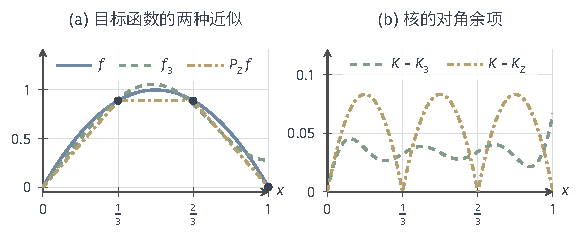
\includegraphics[width=98.2mm]{figures/02-abstract-mathematics/03-function-spaces/tikz/c5-truncation-comparison/figure.pdf}
  \caption{最小值核（$[0,1]$，Lebesgue测度）下三维谱截断与三个中心$Z=\{1/3,2/3,1\}$的投影。(a)~目标$f=4x(1-x)$（实线）、谱截断$f_3$（虚线）与中心投影$P_Zf$（点划线，即过黑点的折线）；(b)~核的对角余项$R_3(x)=K(x,x)-K_3(x,x)$与$P_Z(x)^2=K(x,x)-K_Z(x,x)$，后者在中心处为零但积分更大。}
  \label{fig:rkhs-truncation-comparison}
\end{figure}

在实际计算中，测度常常未知或只能通过样本给出，积分算子的特征函数也无法精确求得。由样本点构造核矩阵并取其谱分解，得到的正是第~\ref{sec:rkhs-center-projection}节的投影核$K_Z$及其有限特征$\Phi_Z$，而不是这里的$K_m$。样本中心与积分谱之间的关系、随机抽取中心或随机特征时的误差，需要另外引入抽样模型来分析；本节的尾和结论不能自动搬到这些数值方法上。

% 第5章第5节：本章小结。

\section{本章小结}
\label{sec:rkhs-summary}

本章从“有限个点值能否作为关于函数的可靠信息”出发，研究点值读取连续的Hilbert函数空间。核与空间之间有双向的对应：空间中每个点的读取有界时，Riesz表示把它写成与核截面$K_x$的内积，核$K(x,z)=\langle K_z,K_x\rangle$对称且半正定；反过来，任何半正定核都唯一地确定一个以它为再生核的空间$H_K$，构造经过系数组合、商去零长度方向、完备化和点值表示四步，核截面的有限组合在其中按核范数稠密。特征映射和核运算把“验证半正定”变成可以操作的检查：写成某个特征向量的内积，或由已知核经非负组合、乘积、换输入、缩放和极限得到。

几项看似相近的性质由不同的条件控制，不能互相代替。固定位置的点值有界由$K(x,x)$给出，全域统一控制要求核的对角有界；读数随位置连续要求核截面距离$\|K_x-K_z\|$随位置趋于零，离散空间$\ell^2(X)$说明前者不蕴含后者。有限观测下，Gram矩阵的零空间只表示系数的冗余，同一函数可以有多种写法；读数相同而函数不同，则来自观测子空间的正交补，它在无限维空间中总存在。投影的唯一性不等于系数的唯一性，最小范数插值由投影几何保证，与系数怎样选取无关。

加入测度后，紧度量空间上的连续半正定核产生紧、自伴、正的积分算子，Mercer定理把核本身展开为一致收敛的谱级数，特征函数在测度全支撑时有唯一的连续代表。核范数在谱坐标下按$1/\lambda_j$加权，于是积分误差小不等于核范数误差小，零谱分量或发散的加权和都把函数排除在$H_K$之外。改变测度会改变特征值和$L^2$坐标，核所定义的内积不变。截断核与截断给定函数控制的是不同的量：前者的误差只依赖核与测度，后者还取决于目标的谱尾；按积分谱截断与按观测中心投影保留的子空间由不同的信息决定，在不同的误差度量下各有优劣。

下一章利用这些空间与表示讨论具体的逼近问题：核截面的有限和能否逼近核空间之外的连续函数，以及怎样用有限个代表统一覆盖整类函数。由核矩阵出发的正则化拟合需要另外给定目标与惩罚，按样本抽取中心的数值近似需要抽样模型，用核比较概率分布则需要把概率测度嵌入核空间；这些问题分别属于优化与模型、统计推断和概率分布的研究，用核比较分布的方法可参考\BookChapterRef{chap:information-theory-and-statistical-geometry}{卷四《数学准备：流形、概率分布与统计推断》“概率分布的分析与优化”章中的最大均值差异}。

